\documentclass[acmtog]{acmart}
\usepackage{algorithm}
\usepackage{algorithmicx}
\usepackage{algpseudocode}
\usepackage{graphicx}
\usepackage{subfigure}
\usepackage{natbib}
\usepackage{listings}
\usepackage{bm}

\def\x{\mathrm{\mathbf{x}}}
\def\y{\mathrm{\mathbf{y}}}
\def\z{\mathrm{\mathbf{z}}}
\def\w{\omega}
\def\p{\mathrm{p}}
\def\pp#1#2{\p_{#1}\rightarrow\p_{#2}}

\definecolor{blve}{rgb}{0.3372549 , 0.61176471, 0.83921569}
\definecolor{gr33n}{rgb}{0.29019608, 0.7372549, 0.64705882}
\makeatletter
\lst@InstallKeywords k{class}{classstyle}\slshape{classstyle}{}ld
\makeatother
\lstset{language=C++,
	basicstyle=\ttfamily,
	keywordstyle=\color{blve}\ttfamily,
	stringstyle=\color{red}\ttfamily,
	commentstyle=\color{magenta}\ttfamily,
	morecomment=[l][\color{magenta}]{\#},
	classstyle = \bfseries\color{gr33n}, 
	tabsize=2
}
\lstset{basicstyle=\small\ttfamily}

% Title portion
\title{CS171 Final Report}

\author{
	Group Number:\quad 1 \\
	Member 1:\quad YiHeng Wu\\
	Member 2:\quad HaiZhao Dai\\
	Member 3:\quad XiaoHan Wu
}

% Document starts
\begin{document}
\maketitle

\vspace*{2 ex}

\section{Introduction}
In this project, we choose to replicate the paper \textit{Spectral and Decomposition Tracking for Rendering Heterogeneous Volumes}.
Volume rendering technique is used in rendering colloid, particals, translucent, and transparent objects. 
For the heterogeneous medium, two unbiased methods based on Monte Carlo methods, delta tracking and weight tracking, are often used.
However, these methods are not efficient in sampling the distance. 
To solve the problem, the authors of the paper proposed decomposition tracking that splits the medium into control component and residual component, which accelerates sampling distance.
\section{Background}
Before the spectral and decomposition tracking, we need to introduce some often-used methods that are the bases of these two methods.

\subsection{Basic Concept}
Considering a participating medium that consists of a collection of particals.
When a ray $\mathbf r(t)=\mathbf o-t\mathbf d$ travels through the medium, it will get absorbed or scattered.
We define $\mu_a$ as the \textit{absorption coefficient} which represents the proportion of radiance that is absorbed by the medium undergoing the respective interaction per unit distance traveled.
Also, $\mu_s$ for the \textit{scattering coefficient}.
The \textit{extinction coefficient} $\mu_t=\mu_a+\mu_s$ indicates the proportion of radiance that loses per unit distance it travels. 
The \textit{ratio} $\alpha=\mu_s/\mu_t$ is the proportion of losed radiance that is scattered.
Generally, these properties are all spatial-varying.

Since there is radiance get out-scattered to other directions, there also is radiance get in-scattered to the direction that ray traveling.
The ray loses radiance in the former event while get compensated from the latter event.
The probability function of the direction that light scattered at a point $\mathbf x$ in the medium is the \textit{phase function} $f_p$.
Generally, it is a function related to the position and the incoming and the outgoing directions, that is:
\begin{equation}
	\begin{aligned}
	f_p:(\mathbf x, \omega_i, \omega_o)\to\mathbb R^+
	\end{aligned}
\end{equation}
The phase function is called isotropic if it scatters the incoming radiance uniformly, that is $f_p=1/(4\pi)$ for all the point in the medium and for all light directions.

Apart from absorption and scattering, volumetric medium can also emit radiance.
The ray traveling through the medium gains radiance from emission.
The four kind of effects are show in fig.\ref{radiative_transfer}.

\begin{figure}[htbp]
	\includegraphics[width=\linewidth]{figure/radiative transfer.png}
	\label{radiative_transfer}
	\caption{Absorption, scattering, and emission of the volumetric medium.}
\end{figure}

If all the properties of the medium are spatial invariant, then the medium is said to be \textit{homogeneous}.
Otherwise, the medium is \textit{heterogeneous}.


\subsection{Radiative Transfer Equation (RTE)}
The radiance transfer equation that describes the change in radiance that travels along direction $\omega$ through a differential volume at point $\mathbf x$ is:
\begin{equation}
	\begin{aligned}
	(\omega\cdot\nabla)L(\mathbf x, \omega)=-\mu_t(\mathbf x)L(\mathbf x, \omega)+\mu_s(\mathbf x)L_s(\mathbf x, \omega)+\mu_a(\mathbf x)L_e(\mathbf x, \omega)\label{RTE}
	\end{aligned}
\end{equation}
where:
\begin{equation}
	\begin{aligned}
	L_s(\mathbf x, \omega)=\int_{\mathcal S^2}f_p(\mathbf x, \omega, \omega')L_i(\mathbf x, \omega')d\omega'
	\end{aligned}
\end{equation}
is the term that measures the in-scattered radiance from other directions distributed on a unit sphere modified by the phase function.

The first term in the RHS of the eq.\eqref{RTE} measures the loss of the radiance when travel through the volume.
The second term measures the gains from incoming radiance.
The third term measures the gains from self-emission.

Integrate both side of the eq.\eqref{RTE}, we get the integral form of RTE:
\begin{equation}
	\begin{aligned}
	L(\mathbf x, \omega)=\int_0^{\infty}T(\mathbf x, \mathbf y)\left[\mu_a(\mathbf y)L_e(\mathbf y, \omega)+\mu_s(\mathbf y)L_s(\mathbf y, \omega)\right]\mathrm dy\label{intRTE}
	\end{aligned}
\end{equation}
where $L(\mathbf x, \omega)$ is the final radiance and $\mathbf y=\mathbf x-y\omega$ is a point in the medium.
The \textit{transmittance} $T(\mathbf x, \mathbf y)$ measures the radiance that is preserved after traveling between two points:
\begin{equation}
	\begin{aligned}
	T(\mathbf x, \mathbf y)=\exp\left(-\int_0^y\mu_t(\mathbf x-s\omega)\mathrm ds\right)
	\end{aligned}
\end{equation}
Here we define the \textit{optical thickness} as $\tau(t)=\int_0^t\mu_t(\mathbf x-s\omega)\mathrm ds$.

For a surface point $\mathbf z=\mathbf x-z\omega$, consider the radiance from the surface, we finally get the volume rendering equation (VRE) (fig.\ref{VRE}):
\begin{equation}
	\begin{aligned}
	L(\mathbf x, \omega)&=\int_0^zT(\mathbf x, \mathbf y)\left[\mu_a(\mathbf y)L_e(\mathbf y, \omega)+\mu_s(\mathbf y)L_s(\mathbf y, \omega)\right]\mathrm dy\\
	&+T(\mathbf x, \mathbf z)L(\mathbf z, \omega)
	\end{aligned}
\end{equation}

\begin{figure}[htbp]
	\includegraphics[width=\linewidth]{figure/volume rendering equation.png}
	\label{VRE}
	\caption{Volume rendering equation}
\end{figure}

where $L(\mathbf z, \omega)$ is the radiance from the surface rendering equation:
\begin{equation}
	\begin{aligned}
	L(\mathbf z, \omega)=L_e(\mathbf z, \omega)+\int_{\mathcal S^2}f_r(\mathbf z, \omega, \omega')L_i(\mathbf z,\omega')(\mathbf n(\mathbf x)\cdot\omega')\mathrm{d}\omega'
	\end{aligned}
\end{equation}
Here, $L_e(\mathbf z, \omega)$ is the direct lighting from the surface point $\mathbf z$ along the direction $\omega$ and $f_r(\mathbf z, \omega, \omega')$ is the bidirectional scattering distribution function (BSDF).
We will discuss the VRE latter as it is the fundamental rendering equation.

\subsection{Basic Tracking Methods}
For simplicity, we only consider evaluating the radiative transfer equation eq.\eqref{intRTE}.
When evaluating the integral-formed RTE, people usually perfer to use Monte Carlo integration.
The Monte Carlo estimator of the equation is:
\begin{equation}
	\begin{aligned}
		\langle L(\mathbf x, \omega)\rangle=\frac{T(\mathbf x, \mathbf y)}{P(\mathbf y)}\left[\mu_a(\mathbf y)L_e(\mathbf y, \omega)+\mu_s(\mathbf y)L_s(\mathbf y, \omega)\right]
	\end{aligned}
\end{equation}

The tracking methods, also referred to as random walk or free-path sampling, require sampling the collision point in the medium and the connect them into a light transfer path.
Given a starting point $\mathbf x_{j}$ ($\mathbf x$ in estimator) and a traveling direction $\omega_{j}$ ($\omega$ in estimator) on the path segment $j$, we need to sample the next collision point $\mathbf x_{j+1}$ ($\mathbf y$ in estimator) and the next sample direction $\omega_{j+1}$.
Sampling direction is easy that we just need to query the phase fuction.
Sampling distance is much harder and in many cases, we need to sample the volumetric medium adaptively.
Here are the frequently-used methods.

\begin{figure}[htbp]
	\includegraphics[width=\linewidth]{figure/tracking.png}
	\label{tracking}
	\caption{
		Three methods for sampling distance in the medium.
		Regular tracking requires the boundary;
		ray marching ignores the boundary, constantly or linearly fitting the extinction coefficient;
		delta tracking adds fictitious medium to the volumetric medium.
	}
\end{figure}

\subsubsection{Analytical Sampling}
Since the transmittance $T(\mathbf x, \mathbf y)$ measures the proportion of the preserved radiance that traveling from $\mathbf x$ to $\mathbf y$ where $\mathbf y=\mathbf x-y\omega$, then we can also consider the transmittance as the probability of a ray that does not interact with the volumetric medium when traveling from $\mathbf x$ to $\mathbf y$.
Usually we can denote $T(\mathbf x, \mathbf y)$ as $T_{\mathbf x}(y)$ which means that the transmittance from the point $\mathbf x$ in the distance $y$.

Let $X$ be a random variable that the ray passes through a distance $y$, then we can get the cumulative distribution function (CDF) of $X$:
\begin{equation}
	\begin{aligned}
		P(X>y)&=T(\mathbf x, \mathbf y)\\
		P(X<y)&=1-T(\mathbf x, \mathbf y)=F_X(y)\\
	\end{aligned}
\end{equation}
By differentiating the CDF, we obtain the probability distribution function (PDF) of $X$:
\begin{equation}
	\begin{aligned}
		P_X(y)&=\frac{dF_X(y)}{dy}=\exp\left(-\int_0^y\mu_t(\mathbf x-s\omega)\mathrm ds\right)\mu_t(\mathbf x-y\omega)\\
		&=T(\mathbf x, \mathbf y)\mu_t(\mathbf y)
	\end{aligned}
\end{equation}

If the extinction coefficient $\mu_t$ is constant, or changing polynomially or exponentially in space, then the distance can be sampled analytically using inverse sampling.
Taking constanct extinction coefficient as example. 
The free-path distance $t$ can be sampled analytically: $t=-\ln(1-\xi)/\mu_t$ where $\xi$ is a sample of the uniform distribution on interval $[0,1]$.
If the inverse of the CDF has no analytically representation, we can apply Newton's method to sample the distance.

\subsubsection{Regular Tracking}
If the medium consists several homogeneous medium with different extinction coefficient, by finding the boundary of the volumetric medium, we can obtain the transmittance and distance sample easily.
Therefore, quickly find the boundary becomes the bottleneck of the performance of regular tracking.

\subsubsection{Ray Marching}
By ignoring the boundary of the volumetric medium, we can sample the volumetric medium within a fix-sized stride. 
This method is efficient for not requiring the boundary.
However, due to the Jensen's inequality, this method is biased.
Though it can be reduced by smaller steps or random jittering, it also increases the cost.

\subsection{Delta Tracking}
Delta tracking is the most famous method used in sampling heterogeneous volumetric medium.
This method is based on reject sampling by introducing the fictitious medium into the real medium.
Therefore we can combine the analytical sampling into this method, and thus making it unbiased.

The fictitious medium in the delta tracking homogenizes the real medium to a constant extinction coefficient medium. We name this coefficient as free-path-sampling coefficient and denote it as $\bar\mu$.
It will not affect the energy of the radiance nor the traveling direction.
Usually people set this bound to the upper bound of the real medium extinction coefficient, that is $\bar\mu=\sup_{\mathbf x}\mu_t(\mathbf x)$. 
The density of the fictitious that fills the gap between the real and the upper bound is denoted as $\mu_n(\mathbf x)$.
By the law of the conservation of energy, we get:
\begin{equation}
	\begin{aligned}
	-\mu_n(\mathbf x)L(\mathbf x, \omega)+\int_{\mathcal S^2}\delta(\omega-\omega')L(\mathbf x, \omega')d\omega'=0
	\end{aligned}
\end{equation}
Plugging it into the eq.\eqref{RTE}, and integraling it, we get:
\begin{equation}
	\begin{aligned}
	&L(\mathbf x, \omega)=\int_0^{\infty}T(\mathbf x, \mathbf y)\\
	&\left[\mu_a(\mathbf y)L_e(\mathbf y, \omega)+\mu_s(\mathbf y)L_s(\mathbf y, \omega)+\mu_n(\mathbf y)L(\mathbf x, \omega)\right]\mathrm dy\label{deltaRTE}
	\end{aligned}
\end{equation}
Here:
\begin{equation}
	\begin{aligned}
	T(\mathbf x, \mathbf y)&=-\exp\left(-\int_0^y\mu_t(\mathbf x-s\omega)+\mu_n(\mathbf x-s\omega)\mathrm ds\right)\\
	&=-\exp\left(-\int_0^y\bar\mu(\mathbf x-s\omega)\mathrm ds\right)\\
	\end{aligned}
\end{equation}
Also, the estimator is modified to:
\begin{equation}
	\begin{aligned}
	\langle L(\mathbf x, \omega)\rangle=\frac{T(\mathbf x, \mathbf y)}{P(\mathbf y)}\left[\mu_a(\mathbf y)L_e(\mathbf y, \omega)+\mu_s(\mathbf y)L_s(\mathbf y, \omega)+\mu_n(\mathbf y)L(\mathbf y, \omega)\right]
	\end{aligned}
\end{equation}

For this estimator, if we substitute the probability function with $P(\mathbf y)=T(\mathbf x, \mathbf y)\bar\mu(\mathbf y)$, then it can be simplfied to:
\begin{equation}
	\begin{aligned}
	\langle L(\mathbf x, \omega)\rangle=\frac{1}{\bar\mu(\mathbf y)}\left[\mu_a(\mathbf y)L_e(\mathbf y, \omega)+\mu_s(\mathbf y)L_s(\mathbf y, \omega)+\mu_n(\mathbf y)L(\mathbf y, \omega)\right]
	\end{aligned}
\end{equation}

Now we introduce probabilities $P_a(\mathbf x)$, $P_s(\mathbf x)$ and $P_n(\mathbf x)$ to allow probabilistically evaluating each of the emission, in-scattering, and null-collision radiance terms:
\begin{equation}
	\begin{aligned}
	&\langle L(\mathbf x, \omega)\rangle=\frac{1}{\bar\mu(\mathbf y)}\\
	&\left[P_a(\mathbf y)\frac{\mu_a(\mathbf y)}{P_a(\mathbf y)}L_e(\mathbf y, \omega)+P_s(\mathbf y)\frac{\mu_s(\mathbf y)}{P_s(\mathbf y)}L_s(\mathbf y, \omega)+P_n(\mathbf y)\frac{\mu_n(\mathbf y)}{P_n(\mathbf y)}L(\mathbf y, \omega)\right]
	\end{aligned}
\end{equation}

The Russian roulette, which is used for unbiased campling, in mathematic is:
\begin{equation}
	\begin{aligned}
	\int_0^1f(x)dx=\int_0^p\frac{f(x)}{p}dx=\int_0^1\mathcal H[x<p]\frac{f(x)}{p}dx
	\end{aligned}
\end{equation}
where $\mathcal H[x]$ is the heavyside function:
\begin{equation}
	\begin{aligned}
	\mathcal H[x] = \begin{cases}
		1& x>0\\
		0& x<0
	\end{cases}
	\end{aligned}
\end{equation}


Then the estimator is:
\begin{equation}
	\begin{aligned}
	&\langle L(\mathbf x, \omega)\rangle=\frac{1}{\bar\mu(\mathbf y)}\\
	&[\int_0^1\mathcal H[\xi_a<P_a(\mathbf y)]\frac{\mu_a(\mathbf y)}{P_a(\mathbf y)}L_e(\mathbf y, \omega)\mathrm d\xi_a\\
	&+\int_0^1\mathcal H[\xi_s<P_s(\mathbf y)]\frac{\mu_s(\mathbf y)}{P_s(\mathbf y)}L_s(\mathbf y, \omega)\mathrm d\xi_s\\
	&+\int_0^1\mathcal H[\xi_n<P_n(\mathbf y)]\frac{\mu_n(\mathbf y)}{P_n(\mathbf y)}L(\mathbf y, \omega)\mathrm d\xi_n]\label{estimator}
	\end{aligned}
\end{equation}

In standard delta tracking, the probability are defined as:
\begin{equation}
	\begin{aligned}
		P_a(\mathbf x)=\frac{\mu_a(\mathbf x)}{\bar{\mu}(\mathbf x)}\quad
		P_s(\mathbf x)=\frac{\mu_s(\mathbf x)}{\bar{\mu}(\mathbf x)}\quad
		P_n(\mathbf x)=\frac{\mu_n(\mathbf x)}{\bar{\mu}(\mathbf x)}
	\end{aligned}
\end{equation}
Note that $\bar\mu\ge\sup\mu_t(\mathbf x)$ should be always satisfied.

Since they are sum to 1, we can simplfy the estimator to cut down the number of sampling random numbers and the branches as the form:
\begin{equation}
	\begin{aligned}
		&\langle L(\mathbf x,\omega)\rangle=\int_0^1\mathcal H[\xi<P_a(\mathbf y)]L_e(\mathbf y,\omega)\\
		&+\mathcal H[P_a(\mathbf y)<\xi<1-P_n(\mathbf y)]L_s(\mathbf y,\omega)\\
		&+\mathcal H[1-P_n(\mathbf y)<\xi]L(\mathbf y,\omega_j)\mathrm d\xi
	\end{aligned}
\end{equation}
Fig.\ref{delta_tracking} (left) shows the properties of the delta tracking.


Here is the pseudo-code of delta tracking:
\begin{algorithm}[H]
	\caption{Pseudocode of Delta Tracking Algorithm}
	\begin{algorithmic}[1]
		\Require
			$\mathbf x$: The collision point; $\omega$: The traveling direction;
		\Ensure
			Next collision point or next travel direction
			\While {true}
				\State $t\gets-\frac{\ln(1-\zeta)}{\bar\mu}$
				\State $\mathbf x\gets\mathbf x-t\times\omega$
				\If {$\xi<\frac{\mu_a(\mathbf x)}{\bar\mu}$}
					\State \Return {$L_e(\mathbf x, \omega)$}
				\ElsIf {$\xi<1-\frac{\mu_n(\mathbf x)}{\bar\mu}$}
					\State $\omega\gets\mathrm{sample}\propto f_p(\omega)$
				\Else {}
					\State \textbf{continue}
				\EndIf
			\EndWhile
	\end{algorithmic}
\end{algorithm}
where $\zeta$ and $\xi$ are random numbers in $[0,1]$.


\begin{figure}[htbp]
	\includegraphics[width=\linewidth]{figure/weighted delta tracking.png}
	\label{delta_tracking}
	\caption{
		The left shows delta tracking and the right shows weighted delta tracking.
		Free-path density is the PDF of the length of the free-path.
		Weight is the adjusted sample weight that used in weighted delta tracking.
		Number of null collsions is the cumulative number of null collsions at distance to the starting position. 
		Density $\times$ weight compensated the effect of the negative extinction coefficient, though it leads to a higher standard deviation.	
	}
\end{figure}

\subsection{Weighted Delta Tracking}
The constrain of the delta tracking is that the free-path-sampleing coefficient should be the close upper bound of the extinction coefficient.
If the extinction coefficient is large at some point while low at others, then delta tracking is inefficient since most of the samples are rejected.
To deal with this problem, two methods are proposed.
One is to partition the space into several subspace with proper extinction coefficient in each subspace.
The spatial partitioning algorithm are kd-tree or grid in practice, we will talk it later.

Another method is weight delta tracking.
It looses the requirement that the free-path-sampleing coefficient can be smaller than the extinction coefficient: $\bar\mu<\mu_t(\mathbf x)$.
This introduces a negative fictitious coefficient which is unreasonable in real-world but efficient for computing.

So we define the probability as:
\begin{equation}
	\begin{aligned}
		P_a(\mathbf x)=\frac{\mu_a(\mathbf x)}{\mu_t(\mathbf x)+|\mu_n(\mathbf x)|}\\
		P_s(\mathbf x)=\frac{\mu_s(\mathbf x)}{\mu_t(\mathbf x)+|\mu_n(\mathbf x)|}\\
		P_n(\mathbf x)=\frac{|\mu_n(\mathbf x)|}{\mu_t(\mathbf x)+|\mu_n(\mathbf x)|}
	\end{aligned}
\end{equation}
And the corresponding estimator is \eqref{estimator}.

And as we can see, if we sample a distance where $\mu_n(\mathbf x)$ is positive,
then the weight will stay 1 no change.
If it is negative, then it means that there are actually two event will happen, absorption or scattering.
But the preset probability is not the actual probability, so we need to adjust the probability using weight.
The weight is always greater equal to 1 theoretically.

Here is the pseudo-code for weighted delta tracking:
\begin{algorithm}[H]
	\caption{Pseudocode of Weighted Delta Tracking Algorithm}
	\begin{algorithmic}[1]
		\Require
			$\mathbf x$: The collision point; $\omega$: The traveling direction;
		\Ensure
			Next collision point or next travel direction
			\State $w\gets1$
			\While {true}
				\State $t\gets-\frac{\ln(1-\zeta)}{\bar\mu}$
				\State $\mathbf x\gets\mathbf x-t\times\omega$
				\If {$\xi<P_a(\mathbf x)$}
					\State \Return {$w\times \frac{\mu_a(\mathbf x)L_e(\mathbf x, \omega)}{\bar\mu P_a(\mathbf x)}$}
				\ElsIf {$\xi<1-P_n(\mathbf x)$}
					\State $\omega\gets\mathrm{sample}\propto f_p(\omega)$
					\State $w\gets w\times \frac{\mu_s(\mathbf x)}{\bar\mu P_s(\mathbf x)}$
				\Else {}
					\State $w\gets w\times \frac{\mu_n(\mathbf x)}{\bar\mu P_n(\mathbf x)}$
				\EndIf
			\EndWhile
	\end{algorithmic}
\end{algorithm}
where $\zeta$ and $\xi$ are random numbers in $[0,1]$.

\section{Decomposition Tracking}
\subsection{Analog Decomposition Tracking}

\begin{table}[htbp]
	\begin{tabular}{c|c}
	\hline
	\textbf{Symbol \& Value}                          & {Description}                               \\ \hline
	$\mu_a^c$                                         & {absorption coef. of control volume}  \\
	$\mu_s^c$                                         & {scattering coef. of control volume}  \\
	$\mu_t^c=\mu_a^c+\mu_s^c$                         & {extinction coef. of control volume}  \\
	$\mu_a^r(\mathbf x)=\mu_a(\mathbf x)-\mu_a^c$     & {absorption coef. of residual volume} \\
	$\mu_s^r(\mathbf x)=\mu_s(\mathbf x)-\mu_s^c$     & {scattering coef. of residual volume} \\
	$\mu_t^r(\mathbf x)=\mu_t(\mathbf x)-\mu_t^c$     & {extinction coef. of residual volume} \\
	$\mu_n(\mathbf x)=\mu-\mu_t^c-\mu_t^r(\mathbf x)$ & {null-collision coef.}                \\ \hline
	\end{tabular}
	\caption{the symbol table for control volume and residual volume}
\end{table}
\begin{algorithm}[H]
	\caption{Pseudocode of Weighted Decomposition Tracking Algorithm}
	\label{weighted_decomposition_tracking_algorithm}
	\begin{algorithmic}[1]
		\Require
		$\mathbf x$: The collision point; $\omega$: The traveling direction;
		\Ensure
		Next collision point or next travel direction
		\State $w\gets1$
		\While {true}
		\State $t\gets-\frac{\ln(1-\zeta)}{\bar\mu}$
		\State $\mathbf x\gets\mathbf x-t\times\omega$
		\State $F\gets0$
		\If {$\xi<(F\gets F+P_a^c(\mathbf x))$}
		\State \Return {$w\times \frac{\mu_a^c(\mathbf x)L_e(\mathbf x, \omega)}{\bar\mu P_a^c(\mathbf x)}$}
		\ElsIf {$\xi<(F\gets F+P_s^c(\mathbf x))$}
		\State $\omega\gets\mathrm{sample}\propto f_p(\omega)$
		\State $w\gets w\times \frac{\mu_s^c(\mathbf x)}{\bar\mu P_s^c(\mathbf x)}$
		\ElsIf {$\xi<(F\gets F+P_a^r(\mathbf x))$}
		\State \Return {$w\times \frac{\mu_a^r(\mathbf x)L_e(\mathbf x, \omega)}{\bar\mu P_a^r(\mathbf x)}$}
		\ElsIf {$\xi<(F\gets F+P_s^r(\mathbf x))$}
		\State $\omega\gets\mathrm{sample}\propto f_p(\omega)$
		\State $w\gets w\times \frac{\mu_s^r(\mathbf x)}{\bar\mu P_s^r(\mathbf x)}$
		\Else{}
		\State $w\gets w\times \frac{\mu_n(\mathbf x)}{\bar\mu P_n(\mathbf x)}$
		\EndIf
		\EndWhile
	\end{algorithmic}
\end{algorithm}
where $\zeta,\psi$ and $\xi$ are random numbers in $[0,1]$.
Delta tracking and weight delta tracking are both useful.
But decomposition tracking is able to reduce the number of queries of the volumetric medium by decomposition the medium into control component and residual component by handling the control volume analytically.

Before introducing the decomposition tracking, let us look a theorem first:
\begin{theorem}
	Let non-negative extinction coefficient $\mu_A(\mathbf x), \mu_B(\mathbf x)$ be combined to $\mu_C(\mathbf x)=\mu_A(\mathbf x)+\mu_B(\mathbf x)$.
	Let $A,B$, and $C$ be independent random variables distributed according to the following CDF $F_X(t)=1-\exp\left(-\int_0^t\mu_X(\mathbf x_s)\mathrm ds\right)$ with $X\in\{A,B,C\}$. The CDFs of $C$ and $\min(A,B)$ are identical. 
\end{theorem}
\begin{proof}
	Let a random variable $D=\min(A,B)$, then:
	\begin{equation}
		\begin{aligned}
			F_D(t)&=P(D\le t)=P(\min(A,B)\le t)=1-P(\min(A,B)> t)\\
			&=1-P(A>t)P(B>t)=1-T_A(t)T_B(t)\\
			&=1-\exp({-\int_0^t\mu_A(\mathbf x_s)ds})\exp({-\int_0^t\mu_B(\mathbf x_s)ds})\\
			&=1-\exp({-\int_0^t\mu_C(\mathbf x_s)ds})\\
			&=F_C(t)
		\end{aligned}
	\end{equation}
	which means that the CDFs of $C$ and $\min(A,B)$ are identical. 
\end{proof}

\begin{algorithm}[H]
	\caption{Pseudocode of Decomposition Tracking Algorithm}
	\label{decomposition_tracking_algorithm}
	\begin{algorithmic}[1]
		\Require
			$\mathbf x$: The collision point; $\omega$: The traveling direction;
		\Ensure
			Next collision point or next travel direction
			\While {true}
				\State $t^c\gets-\frac{\ln(1-\zeta)}{\mu_t^c}$
				\State $t^r\gets0$
				\While {true}
					\State $t^r\gets t^r-\frac{\ln(1-\psi)}{\bar\mu-\mu_t^c}$
					\If {$t^r>t^c$}
						\State $\mathbf x\gets\mathbf x-t^c\times\omega$
						\If {$\xi<\frac{\mu_a^c(\mathbf x)}{\mu_t^c}$}
							\State \Return {$L_e(\mathbf x, \omega)$}
						\Else
							\State $\omega\gets\mathrm{sample}\propto f_p(\omega)$
							\State \textbf{break}
						\EndIf
					\Else {}
						\If {$\xi<\frac{\mu_a^r(\mathbf x)}{\bar\mu-\mu_t^c}$}
							\State $\mathbf x\gets\mathbf x-t^r\times\omega$
							\State \Return {$L_e(\mathbf x, \omega)$}
						\ElsIf {$\xi<1-\frac{\mu_n(\mathbf x)}{\bar\mu-\mu_t^c}$}
							\State $\mathbf x\gets\mathbf x-t^r\times\omega$
							\State $\omega\gets\mathrm{sample}\propto f_p(\omega)$
							\State \textbf{break}
						\EndIf
					\EndIf
				\EndWhile
			\EndWhile
	\end{algorithmic}
\end{algorithm}
where $\zeta,\psi$ and $\xi$ are random numbers in $[0,1]$.

Then we can sample the free-path in both control volume and residual volume.
And find the smaller distance for the sampling.
Here we can combine the analytical sampling and delta tracking to form the decomposition tracking (see the algorithm.\ref{decomposition_tracking_algorithm}).

\subsection{Weighted Decomposition Tracking}
The estimator now is:
\begin{equation}
	\begin{aligned}
	&\langle L(\mathbf x, \omega)\rangle=\frac{1}{\bar\mu(\mathbf y)}\\
	&[\int_0^1\mathcal H[\xi_a^c<P_a^c(\mathbf y)]\frac{\mu_a^c(\mathbf y)}{P_a^c(\mathbf y)}L_e(\mathbf y, \omega)\mathrm d\xi_a^c\\
	&+\int_0^1\mathcal H[\xi_a^r<P_a^r(\mathbf y)]\frac{\mu_a^c(\mathbf y)}{P_a^r(\mathbf y)}L_e(\mathbf y, \omega)\mathrm d\xi_a^r\\
	&+\int_0^1\mathcal H[\xi_s^c<P_s^c(\mathbf y)]\frac{\mu_s^c(\mathbf y)}{P_s^c(\mathbf y)}L_s(\mathbf y, \omega)\mathrm d\xi_s^c\\
	&+\int_0^1\mathcal H[\xi_s^r<P_s^r(\mathbf y)]\frac{\mu_s^c(\mathbf y)}{P_s^r(\mathbf y)}L_s(\mathbf y, \omega)\mathrm d\xi_s^r\\
	&+\int_0^1\mathcal H[\xi_n<P_n(\mathbf y)]\frac{\mu_n(\mathbf y)}{P_n(\mathbf y)}L(\mathbf y, \omega)\mathrm d\xi_n]
	\end{aligned}
\end{equation}
Similar to what we did in weighted delta tracking, we define the probability of each term:
\begin{equation}
	\begin{aligned}
		P_a^c=P_cP_{a|c}=\frac{\mu_t^c}{\bar\mu}\frac{\mu_a^c}{\mu_t^c}=\frac{\mu_a^c}{\bar\mu}\\
		P_s^c=P_cP_{s|c}=\frac{\mu_t^c}{\bar\mu}\frac{\mu_s^c}{\mu_t^c}=\frac{\mu_s^c}{\bar\mu}
	\end{aligned}
\end{equation}
And for the sake of the sum of the probability to be one:
\begin{equation}
	\begin{aligned}
		P_a^r(\mathbf x)=\left(1-\frac{\mu_t^c}{\bar\mu}\right)\frac{|\mu_a^r(\mathbf x)|}{|\mu_a^r(\mathbf x)|+|\mu_s^r(\mathbf x)|+|\mu_n(\mathbf x)|}\\
	P_s^r(\mathbf x)=\left(1-\frac{\mu_t^c}{\bar\mu}\right)\frac{|\mu_s^r(\mathbf x)|}{|\mu_a^r(\mathbf x)|+|\mu_s^r(\mathbf x)|+|\mu_n(\mathbf x)|}\\
	P_n(\mathbf x)=\left(1-\frac{\mu_t^c}{\bar\mu}\right)\frac{|\mu_n(\mathbf x)|}{|\mu_a^r(\mathbf x)|+|\mu_s^r(\mathbf x)|+|\mu_n(\mathbf x)|}
	\end{aligned}
\end{equation}

So by combining the weighted delta tracking and decomposition tracking, we get the weighted decomposition tracking algorithm (algorithm.\ref{weighted_decomposition_tracking_algorithm}).

\subsection{Analysis}
The decomposition tracking is efficient if the upper bound of the control component is high.
If the control component is too low, it is not efficient compared to the original delta tracking since it need to compute one more sample.
Furthermore, since the analog decomposition relies on delta tracking, it can handle only a single wavelength.
We will deal with this problem by spectral tracking.



\section{Spectral Tracking}
Usually, when we talk about the radiance, we have accepted the fact that:
\begin{equation}
	\begin{aligned}
		L(\mathbf x, \omega)=\int_{\lambda}L(\mathbf x, \omega, \lambda)\mathrm d\lambda
	\end{aligned}
\end{equation}
where $\lambda$ is the wavelength of the ray.

In practice and for the photo-realistic, the properties of the volumetric medium are wavelength-dependent.
Obviously, we can not cover all the wavelength of the ray.
But the mixture of the red, green, and blue (RGB) color can recover all the color.
So using a vector of $N_{\lambda}$ wavelength is enough.

We define a single distribution for sampling collisions and counteract the discrepancy between this distribution and the true, per wavelength free-path distribution by reweighting just like weighted delta tracking.
Ideally, to keep the variance low and reduce the number of sampling, we should set the free-path-sampling coefficient $\bar\mu=\sup_{\lambda}\mu_t(\mathbf x, \lambda)$.

Obviously, we can not set a uniform probabilities to cancel out the $\mu_{\star}(\mathbf x, \lambda)/\bar\mu$.
But the author proposed to use the maximum and the average-based coefficient for the probability.

The maximum probability is:
\begin{equation}
	\begin{aligned}
		P_a(\mathbf x)&=\max_{\lambda}(|\mu_a(\mathbf x)|)c^{-1}\\
		P_s(\mathbf x)&=\max_{\lambda}(|\mu_s(\mathbf x)|)c^{-1}\\
		P_n(\mathbf x)&=\max_{\lambda}(|\mu_n(\mathbf x)|)c^{-1}\\
		c&=\max_{\lambda}(|\mu_a(\mathbf x)|)+\max_{\lambda}(|\mu_s(\mathbf x)|)+\max_{\lambda}(|\mu_n(\mathbf x)|)\\
	\end{aligned}
\end{equation}
This will allow the number of local collision to be no more than 3 no matter how many wavelength we trace.

Next is average-based probability:
\begin{equation}
	\begin{aligned}
		P_a(\mathbf x)&=\mathrm {avg}_{\lambda}(|\mu_a(\mathbf x)w(\mathbf X,\lambda)|)c^{-1}\\
		P_s(\mathbf x)&=\mathrm {avg}_{\lambda}(|\mu_s(\mathbf x)w(\mathbf X,\lambda)|)c^{-1}\\
		P_n(\mathbf x)&=\mathrm {avg}_{\lambda}(|\mu_n(\mathbf x)w(\mathbf X,\lambda)|)c^{-1}\\
		c&=\sum_{\star}\mathrm {avg}_{\lambda}(|\mu_\star(\mathbf y)w(\mathbf X,\lambda)|)
	\end{aligned}
\end{equation}
where $\mathbf X$ is the weight from previous path segment.
We call this histroy-aware method.
This will allow the number of local collision to be no more than $N_{\lambda}$.

By modifying the weight delta tracking algorithm, we can get:
\begin{algorithm}[H]
	\caption{Pseudocode of Spectral Tracking Algorithm}
	\begin{algorithmic}[1]
		\Require
			$\mathbf x$: The collision point; $\omega$: The traveling direction;
		\Ensure
			Next collision point or next travel direction
			\State $\hat w\gets(1,\dots,1)_{N_{\lambda}}$
			\While {true}
				\State $t\gets-\frac{\ln(1-\zeta)}{\bar\mu}$
				\State $\mathbf x\gets\mathbf x-t\times\omega$
				\If {$\xi<P_a(\mathbf x)$}
					\State \Return {$\hat w\times \frac{\hat\mu_a(\mathbf x)\hat L_e(\mathbf x, \omega)}{\bar\mu P_a(\mathbf x)}$}
				\ElsIf {$\xi<1-P_n(\mathbf x)$}
					\State $\omega\gets\mathrm{sample}\propto f_p(\omega)$
					\State $\hat w\gets \hat w\times \frac{\hat\mu_s(\mathbf x)}{\bar\mu P_s(\mathbf x)}$
				\Else {}
					\State $\hat w\gets \hat w\times \frac{\hat\mu_n(\mathbf x)}{\bar\mu P_n(\mathbf x)}$
				\EndIf
			\EndWhile
	\end{algorithmic}
\end{algorithm}

In practice, these probabilities reduce the magnitude of undesired color noise and avoid bright chromatic outliers.

\subsection{Residual Ratio Tracking}
Ratio tracking and residual tracking,a way that is able to handle media with wavelength dependent extinction, can be combined to compute unbiased,low-variance transmittance estimates in general heterogeneous media.To be more specfic,ratio tracking is to leverage the information discovered during the tracking more efficiently instead of deducing “just” a binary answer,finally provides a piecewise constant approximation to the transmittance function.Residual tracking,in the other hand,is complementary to delta tracking and ratio tracking and combines numerical estimation with an analytic approximation, yielding a piecewise exponential solution.
\subsubsection{Ratio Tracking}
\paragraph {\textbf{Definition}}
Ratio tracking is defined by following rules: 1.Replacing the Russian roulette by a weight that is equal to the probability of colliding with a fictitious particle. 2.Continuing the random walk until it reaches the end-point of the ray instead of probabilistically terminating the random walk at one of tentative collision points. 3.keeping track of the joint probability of colliding points with fictitious particles at all the preceding tentative collisions during the construction.By following the above rules, we can define the transmittance when reading d as:
\begin{equation}
	\begin{aligned}
		T(d)=\prod_{i=1}^{K}(1-\frac{\mu(x_{i})}{\bar{\mu}})
	\end{aligned}
\end{equation}
The multiplicand in the product represents the ratio of fictitious to all particles at collision point $x_i$.
\\Algorithm 1 is the pseudo-code of ratio tracking:
\begin{algorithm}[h]
	\caption{Pseudocode of the ratio tracking estimator of transmittance
		along a ray with origin $o$, direction $\omega$, and length $d$.}
	\begin{algorithmic}[1]
		\Function{RatioTrackingEstimator}{$o,\omega,d$}
		\State $t=0$
		\State $T=1$
		\State \textbf{do:}
		\State  \qquad$\zeta=rand() $
		\State  \qquad$t=t-\frac{log(1-\zeta)}{\bar{\mu}} $
		\State  \qquad\textbf{if} $t\geq d:$ \textbf{break}
		\State  \qquad$T = T *(1-\frac{\mu(o+t*\omega)}{\bar{\mu}}) $
		\State \textbf{while} true
		\State \textbf{return} T
		\EndFunction  
	\end{algorithmic}
\end{algorithm}\\

\paragraph {\textbf{Unbiasedness of Ratio Tracking}}
The unbiasedness of Ratio Tracking can be demonstrated if it follows the following equation:
\begin{equation}
	\begin{aligned}
		E[T] = exp(-\int_{0}^{d}\mu(x)dx) = T(d)
	\end{aligned}
\end{equation}
Now we try to prove that conclusion.
Denoting $tau_i$ realizations of $T_i$,the expected value of T can be written as:
\begin{equation}
	\begin{aligned}
		E[T] = E[\sum_{i=0}^{\infty}T_i]=\sum_{i=0}^{\infty}E[T_i]=\sum_{i=0}^{\infty}\int_{i=0}^{\infty}\tau_i dP(\tau_i)
	\end{aligned}
\end{equation}
To list $T_0$ and $T_1$ as example,$T_0$ represents all realizations with the first tentative free flight distance $S_1$ already exceeding $d$.Since the value of $T_0$ equals to 1,the expected value reduces to the probability of $S_1$ taking on values greater than $d$:
\begin{equation}
	\begin{aligned}
		E[T_0] = P(S_1> d) = \int_{d}^{\infty}\tau_i dP(\tau_i)p_s(x)dx = exp(-\bar{\mu}d)
	\end{aligned}
\end{equation}
In the case of $T_1$, which represents events where $S_1 \leq d$ and $S_2 \geq -S_1$,then the expectancy of $T_1$ reads:
\begin{equation}
	\begin{aligned}
		E[T_1] &= \int_{0}^{d}\iota(x) P(S_2>d-x)dP(S_1\leq x)\\
		&= \int_{0}^{d}\iota(x_1) P_s(x_1)\int_{d-x1}^{\infty}p_s(x_2)dx_2dx_1\\
		&= \int_{0}^{d}\iota(x_1) \bar{\mu} exp(-\bar{\mu x_1})exp(-\bar \mu(d-x_1))dx_1\\
		&=\bar{\mu}exp(-\bar{\mu}d)\int_{0}^{d}\iota(x)dx\\
	\end{aligned}
\end{equation}
Then we can analogously express the expected value of $T_k$, where represents realizations that satisfy $C_k \leq d$ and $C_k+1 >d-C_k$,as:
\begin{equation}
	\begin{aligned}
		E[T_k] &= \int_{0}^{d}\iota(x_1) P_s(x_1)\int_{0}^{d-x_1}\iota(x_1+x_2) P_s(x_2)...\\&...
		\int_{0}^{d-\sum_{j=1}^{k-1}x_j}\iota (\sum_{j=1}^{k}x_j)p_s(x_k)\\
		&\times\int_{d-\sum_{j=1}^{k-1}x_j}^{\infty}p_s(x_{k+1})dx_{k+1}dx_k...dx_2dx_1\\
		&=\int_{0}^{d}\iota(x_1)\int_{0}^{d-x_1}\iota(x_1+x_2)...\int_{0}^{d-\sum_{j=1}^{k-1}x_j}\iota (\sum_{j=1}^{k}x_j) \\
		&\times\int_{d-\sum_{j=1}^{k-1}x_j}^{\infty}\bar{\mu}^kexp(-\bar{\mu}(x_1+...x_k+(d-\sum_{j=1}^{k}x_j)))\\&dx_{k+1}dx_k...dx_2dx_1\\
		&=\bar{\mu}^kexp(-\bar{\mu}d)\int_{0}^{d}\iota(x_1)\int_{0}^{d-x_1}\iota(x_1+x_2)...\\
		&...\int_{0}^{d-\sum_{j=1}^{k-1}x_j}\iota (\sum_{j=1}^{k}x_j)dx_k...dx_2dx_1\\
	\end{aligned}
\end{equation}
Then we replace $z_i$ for $\sum_{j=0}^{i}x_j$ to rewrite the equation as:
\begin{equation}
	\begin{aligned}
		E[T_k]&=\bar{\mu}^kexp(-\bar{\mu}d)\int_{0}^{d}\iota(z_1)\int_{0}^{d-z_1}\iota(z_2)...\\
		&...\int_{0}^{d-z_{k-1}}\iota (z_k)dz_k...dz_2dz_1\\
	\end{aligned}
\end{equation}
The multiple integrals integrate $\prod_{j=1}^{k}\iota(z_j) $ over a k-dimensional simplex, which can be written concisely as:
\begin{equation}
	\begin{aligned}
		E[T_k]&=\bar{\mu}^kexp(-\bar{\mu}d)\frac{(\int_{0}^{d}\iota(x)dx)^k}{k!}
	\end{aligned}
\end{equation}
Finally,we express the expected value of T as following:
]\begin{equation}
	\begin{aligned}
		E[T]&=\sum_{k=0}^{\infty}E[T_k]\\
		&=\sum_{k=0}^{\infty}\bar{\mu}^kexp(-\bar{\mu}d)\frac{(\int_{0}^{d}\iota(x)dx)^k}{k!}\\
		&=exp(-\bar{\mu}d)\sum_{k=0}^{\infty}\frac{(\bar{\mu}\int_{0}^{d}\iota(x)dx)^k}{k!}\\
		&=exp(-\bar{\mu}d)exp(\bar{\mu}\int_{0}^{d}1-\frac{\mu(x)}{\bar{\mu}}dx)\\
		&=exp(-\int_{0}^{d}\bar{\mu}dx)exp(\int_{0}^{d}\bar{\mu}-\mu(x)dx)\\
		&=exp(-\int_{0}^{d}{\mu}(x)dx)
	\end{aligned}
\end{equation}
Though ratio tracking is unbiased, its weakness is also obvious:the expected number of steps required to reach the endpoint of the ray is high,which directly depends on the value of the majorant extinction coefficient.That's why we introduce residual tracking.
\subsubsection{Residual Tracking}
\paragraph {\textbf{Definition}}
Before introducing the definition of residual trakcing, we first analyize the transmittion function,where $\mu_c(x)$ is the extinction coefficient which is a simplified version of the original $\mu(x)$ that enables expressing the optical thickness up to distance $d$ in closed form $\tau_c(d)$:
]\begin{equation}
	\begin{aligned}
		T(d)&=exp(-\int_{0}^{d}\mu(x)dx)\\
		&=exp(-\int_{0}^{d}\mu_c(x)+\mu(x)-\mu_c(x)dx)\\
		&=exp(-\tau_c(d)) exp(-\int_0^d\mu(x)-\mu_c(x)dx)
	\end{aligned}
\end{equation}
The first exponential term, referred to as the control transmittance $T_c(d)$, represents a coarse approximation of $T(d)$, which is computed using the simplified extinction coefficient $\mu_c$. The second exponential then serves as a correction that accounts for the difference between the control and the actual transmittance. We denote
this exponential as the residual transmittance$ T_r$ and refer to the integrand as the residual extinction coefficient $\mu_r(x) = \mu(x)-\mu_c(x)$.
There is also one thing worth noticing---- in certain situations—depending on the value of $\mu_c(x)$—the residual extinction may be negative.
\\Algorithm 2 is the pseudo-code of residual ratio tracking:
\begin{algorithm}[h]
	\caption{Pseudocode of the residual ratio tracking estimator for sampling transmittance along a ray with origin $o$, direction $\omega$, and length $d$.}
	\begin{algorithmic}[1]
		\Function{ResidualRatioTrackingEstimator}{$o,\omega,d$}
		\State $t=0$
		\State $T_c=exp(-\mu_c*d)$
		\State $T_r=1$
		\State \textbf{do:}
		\State  \qquad$\zeta=rand() $
		\State  \qquad$t=t-\frac{log(1-\zeta)}{\bar{\mu_r}} $
		\State  \qquad\textbf{if} $t\geq d:$ \textbf{break}
		\State  \qquad$T_r = T_r *(1-\frac{\mu(o+t*\omega)-\mu_c}{\bar{\mu_r}}) $
		\State \textbf{while} true
		\State \textbf{return} $T_c*T_r$
		\EndFunction  
	\end{algorithmic}
\end{algorithm}\\
\paragraph{\textbf{Expression}}
According to the equation metioned before, we can obtain the residual ratio tracking estimator as below:
]\begin{equation}
	\begin{aligned}
		\left<T_r(d)\right>_{RR} = \prod_{i=1}^{K}(1-\frac{\mu_r(x_i)}{\bar{\mu_r}}) = \prod_{i=1}^{K}(1-\frac{\mu(x_i)-\mu_c}{\bar{\mu_r}})
	\end{aligned}
\end{equation}
As our goal is to minimize the tracking cost by prolonging the tentative free-flight distances, it yields to finding the smallest $\bar{\mu_r}$ that still avoids negative multiplicands,which would prevent convergence of the above estimator.To ensure that $\mu_r(x)/\bar{\mu_r} \leq 1$, we set $\bar{\mu_r} = max(|\mu_r(x)|;0\leq x \leq d)$,i.e. the maximum absolute difference between $\mu(x)$ and $\mu_c$ along the ray.


For different values of $\mu_c$, the visiulization of them is totally different,shown in the following figure, where the bright regions correspond to cases when the residual transmittance takes on values higher than 1 to correct for the overly low control transmittance.
\begin{figure}[htbp]
	\includegraphics[width=\linewidth]{vis.PNG}
	\label{Residual ratio tracking}
	\caption{
		Residual ratio tracking in a simple procedural volume with the control transmittance (a) computed using the minimum (top), the average (middle), and the maximum (bottom) extinction coefficient in the volume. The residual transmittance (b) used to compute the product (c) was estimated using 4 trackings only to
		emphasize the noise typical for each control extinction
	}
\end{figure}
\begin{itemize}
	\item if $\mu_c = \mu_{min} = min(\mu(x));0 \leq x \leq d)$,i.e. the control extinction is underestimating, the control transmittance systematically overestimates the real transmittance
	\item if $\mu_c = \mu_{avg} = avg(\mu(x));0 \leq x \leq d)$,the control extinction
	along the ray matches the real extinction on average. The residual tracking thus corrects only for the local over- and underestimation of the control transmittance w.r.t. the real transmittance along the ray.
	\item if $\mu_c = \mu_{max} = max(\mu(x));0 \leq x \leq d)$,the control transmittance
	systematically underestimates the real transmittance and the residual tracking thus needs to produce values greater than 1 to scale the control up.
\end{itemize}
\paragraph {\textbf{Unbiasedness of Residual Ratio Tracking}}
The unbiasedness of Residual Ratio Tracking can be demonstrated if it follows the following equation:
\begin{equation}
	\begin{aligned}
		E[T] = exp(-\int_{0}^{d}\mu(x)-\mu_cdx) = \frac{T(d)}{exp(-\mu_cd)}
	\end{aligned}
\end{equation}
Now we try to prove that conclusion.As tge proof is very similar, we can directly mimic the above proof:
\begin{equation}
	\begin{aligned}
		E[T]&=exp(-\bar{\mu_r}d)\sum_{k=0}^{\infty}\frac{(\bar{\mu_r}\int_{0}^{d}\iota(x)dx)^k}{k!}\\
		&=exp(-\bar{\mu_r}d)exp(\bar{\mu_r}\int_{0}^{d}1-\frac{\mu(x)-\mu_c}{\bar{\mu_r}}dx)\\
		&=exp(-\int_{0}^{d}\bar{\mu_r})exp(\int_{0}^{d}\bar{\mu_r}-(\mu(x)-\mu_c)dx)\\
		&=exp(-\int_{0}^{d}{\mu dx}(x)-\mu_cdx)
	\end{aligned}
\end{equation}
\subsection{Adaptive and unbiased sampling using kd-tree based space partitioning}
As it's a time-consuming process to find a new scattering event in inhomogeneous participating meadia,we use an adaptive and unbiased sampling technique using kd-tree based space. partitioning. During preprocessing, it partitions the analytical space (the bounding
box of the medium) into sub-spaces (partitions,presented in kd-tree) according to the spatial variation of the mean free path in the medium. During rendering, the locations
of the scattering events are determined adaptively using the kd-tree.
\\Here is the pseudo-code of WoodcockTracking and kdTreeFreePathSampling:
\begin{algorithm}[h]
	\caption{Pseudocode of WoodcockTracking Algorithm}
	\begin{algorithmic}[1]
		\Require
		$x_0,\vec{\omega}$:The ray starting at $x_0$ in direction $\vec{\omega}$\\
		$k_M$:The majorant extinction coefficient\\
		$(d_{min},d_{max}]$:The interval of the ray to evaluate
		\Ensure
		The free path d to the next scattering event
		\State $d\gets d_{min}$-ln(1-rand())/$k_M$ 
		\While {$d\leq d_{max}\land k(x_0+d\vec{\omega})/k_M<rand()$}
		\State $d\gets d$-ln(1-rand())/$k_M$ 
		\EndWhile
		\State \Return {d}
	\end{algorithmic}
\end{algorithm}\\

\begin{algorithm}[h]
	\caption{Pseudocode of kdTreeFreePathSampling Algorithm}
	\begin{algorithmic}[1]
		\Require
		$x_0,\vec{\omega}$:The ray starting at $x_0$ in direction $\vec{\omega}$
		\Ensure
		The free path d to the next scattering event
		\While {true}
		\State $kdTreeNode\ p\gets findNextLeafNode()$ 
		\If {$p=nil$}
		\State \Return {INFINITY} \EndIf
		\State $(d_{min},d_{max})\gets intersectionBetweenRayAndNode(p)$ 
		\State $k_M\gets majorantExtinctionCoefficientStoredIn(p)$ 
		\State $d\gets WoodcockTracking(x_o,\vec{\omega},k_M,d_{min},d_{max})$ 
		\State $d_{isect}\gets INFINITY$
		\If {$intersectionWithObjectSurfaces(x_0,\vec{\omega},p$)}
		\State $d_{isect} \gets distanceToTheIntersection()$ \EndIf
		\If {$d \geq d_{isect}$}
		\State \Return {IntersectionEvent} \EndIf
		\If {$d < d_{max}$}
		\State \Return {d} \EndIf
		\EndWhile
	\end{algorithmic}
\end{algorithm}
\subsubsection{Unbiased Sampling and Space Partitioning}
\paragraph{\textbf{Strategy}}
Suppose the ray starting at $x_0$ in direction $\vec{\omega}$ passes through two adjacent partitions i and j, with $k_M^{(i)}$ and $k_M^{(j)}$ being their majorant extinction coefficients. Let the distances from $x_0$ to the intersections with those partitions be s, q, and t.\\
First,to sample the free path in the interval $(s,t]$,we first deal with the $(s,q])$ by using WoodcockTracking Algorithm,and if the free pathexceeds q, we rewind the free path back to q and proceed to interval $(q,t]$ and use that algorithm again.By rewinding the free path back to q, we can ensure the unbiasedness of the sampling.
\paragraph{\textbf{Proof of Unbiasedness}}
To prove unbiasedness, we need to show taht we can obtain the free path d with probability:
\begin{equation}
	\begin{aligned}
		&P(x'=x_0 + d\vec{\omega}\land s<d\leq t) = e^{-\tau(x_0+s\vec{\omega},x')}k(x')\\
		&P(d>t)= e^{-\tau(x_0+s\vec{\omega},x_0+t\vec{\omega})}
	\end{aligned}
\end{equation}
First, we obtain $d_1$ during the sampling for the first interval (s,q] with the probability:
\begin{equation}
	\begin{aligned}
		&P(x'=x_0 + d_1\vec{\omega}\land s<d_1\leq q) = e^{-\tau(x_0+s\vec{\omega},x')}k(x')\\
		&P_1(d_1>q)= e^{-\tau(x_0+s\vec{\omega},x_0+q\vec{\omega})}
	\end{aligned}
\end{equation}
Similarily, we obtain $d_2$ during the sampling for the second interval (q,t]
\begin{equation}
	\begin{aligned}
		&P(x'=x_0 + d_2\vec{\omega}\land q<d_2\leq t) = e^{-\tau(x_0+q\vec{\omega},x')}k(x')\\
		&P_1(d_2>t)= e^{-\tau(x_0+q\vec{\omega},x_0+t\vec{\omega})}
	\end{aligned}
\end{equation}
Since the sampling for the second interval is executed if and only if $d_1$ exceeds q during the sampling for the first interval, we obtain
\begin{equation}
	\begin{aligned}
		P(x'=x_0 + d\vec{\omega}\land s<d\leq q)
		&=P_1(x'=x_0 + d\vec{\omega}\land s<d\leq q)\\
		&= e^{-\tau(x_0+s\vec{\omega},x')}k(x')\\
		P(x'=x_0 + d\vec{\omega}\land q<d\leq t)
		&=P_1(d_1>q)P_2(x'=x_0 + d\vec{\omega}\land q<d\leq t)\\
		&=e^{-\tau(x_0+s\vec{\omega},x_0+q\vec{\omega})}e^{-\tau(x_0+q\vec{\omega},x')}k(x')\\
		&=e^{-\tau(x_0+s\vec{\omega},x')}k(x')\\
		P(d>t) = P_1(d>q)P_2(d>t)
		&=e^{-\tau(x_0+s\vec{\omega},x_0+q\vec{\omega})}e^{-\tau(x_0+q\vec{\omega},x_0+t\vec{\omega})}\\
		&=e^{-\tau(x_0+s\vec{\omega},x_0+t\vec{\omega})}
	\end{aligned}
\end{equation}
\subsubsection{Unbiased Sampling and Space Partitioning}
The performance of the sampling technique shown in previous section highly depends on the partitioning. If we partition a nearly homogeneous interval, an additional iteration is required to rewind the free path to q when proceeding to the adjacent interval, and this
would be a waste compared to the case with no partitioning. On the other hand, we can have more benefit, if $k_M^{(i)}$ in a partition is much smaller than kM for the entire space. These observations would give us a stopping criterion for the partitioning process, as well as a decision criterion for the partitioning location q.

\section{Implementation}
The implementation is based on HW3 and HW4 of YiHengWu, to which our group members add a lot more functions and classes so that it can fit the condition of volume rendering.
It follows the PBRT naming style for variables and functions so that those who are familiar with PBRT will find it comfortable to read the code.\par
The PBRT-style framework splits the tracer into independent parts: 
shape, primitive, aggregate, sampler, distribution, scattering, material, texture, light, medium.
These information accompanied with the camera are recorded in the scene settings.
The scene is finally rendered by the integrator and an image is outputted.\par
We assume that the readers are familiar with PBRT so we will only focus on medium, integrator and aggregate.

\subsection{Volume}
See `medium/volume.h' and `medium/volume.cpp' for more details.\par
The volume framework is based on OpenVDB, 
thus a volume is simply a OpenVDB grid with some interfaces to access the internal value.
A smoke can be mostly described by its density with a VDB float grid.
A problem is that the grid is described in an unsigned integer coordinate (grid coordinate) so that
rays should be transformed from the world coordinate to the grid coordinate before tracking.
That is why `LocalToGrid()' is a necessary virtual function of `class Volume'.
\begin{lstlisting}
	class Volume:
	public:
	virtual Transform LocalToGrid() const = 0;
\end{lstlisting}
We will focus on the child class `class VolumeFloatGrid' and its child class `class VolumeFloatKDTree'.\par
The reason why we also need a KDTree is that 
simply using the uniform grid for decomposition tracking will always result in bad performance 
because the minimum value of grid, which is chosen as $\mu_t^c$, is always very small.
So we use a KDTree to split the grid into blocks where the minimum value inside each block is expected to be higher.
Our implementation of the KDTree is based on the article introduced above.
\begin{lstlisting}
	class VolumeFloatGrid : public Volume;
	class VolumeFloatKDTree : public VolumeFloatGrid;
\end{lstlisting}

\subsubsection{Grid}
The implementation of `class VolumeFloatGrid' is quite simple.
It simply provides interfaces between our framework and OpenVDB data structure.
Information about the grid including the max and min value and the boundary are recorded as fields to enable fast accessing.

\subsubsection{KDTree}
The KDTree is the child class of the grid, with node-level fields including the max and min value, split axis and split position.
Information about a node is compressed and recorded into 64 bits.
The format of the tree is shown here.
\begin{figure}[H]
	\includegraphics[scale=0.065]{pictures/kdTree format.png}
	\centering
	\caption{KDTree node format.}
\end{figure}
The lowest two bits (split axis) is used to indicate whether a node is a internal or leaf node.
For internal nodes, split axis $\in { 0, 1, 2 }$ indicating ${ x, y, z }$ axis.
For leaf nodes, the lowest two bits are fixed to $3$.\par
You may have noticed that split axis shares two bits with max value so that
for leaf nodes, the lowest two bits of the max value is always `0b11', 
which results in some acceptable errors but achieves great speedup.\par
You may also have noticed that parent nodes do not record the index of their child nodes.
This makes our kdTree different from PBRT.
We compressed the kdTree into a heap where children of node at array index $i$ are located at $i<<1$ and $(i<<1)+1$.
We chose this design to compress the node into 64-bits, making it more cache-friendly for 64-bit-cacheline systems.\par
Following this format, `class VolumeFloatKDTree' provides 4 inline functions to
get split axis, split position of internal nodes and max, min value of leaf nodes.
Here shows the interfaces, where `idx' is the index of the kdTree array with 64-bit stride.
\begin{lstlisting}
	class VolumeFloatKDTree : public VolumeFloatGrid:
	public:
	inline int KDTreeSplitAxis(int idx) const;
	inline int KDTreeSplitPos(int idx) const;
	inline int KDTreeMaxValue(int idx) const;
	inline int KDTreeMinValue(int idx) const;
	private:
	void* kdTree;
\end{lstlisting}
Building of the KDTree is based on the article introduced above.
Since the implementation is simple, it will not be discussed here.

\subsection{Medium}
See `medium/medium.h', `medium/medium.cpp' for more details.\par
This section will focus on the interface design of the medium system.
Readers can skip this part if they are familiar with PBRT.\par
As we have fully explained, the volume path tracing procedure primarily needs 3 building blocks:
sampling scattering distance, evaluating transmittance and sampling scattering direction.\par
\subsubsection{Sample Distance}
Weighed delta tracking and weighed decomposition tracking are used.
Since these two solutions are based on reject sampling, a random number generator (or a sampler in our framework) is needed.
The current weight is also given as a parameter, which will be updated during samples.
Sampling results including the position is recorded in a `MediumInteraction'.
Here is the interface.
\begin{lstlisting}
	class Medium:
	public:
	virtual Spectrum Sample(
	const Ray& rayWorld,  // World-coord ray
	Sampler& sampler,     // Random generator
	Spectrum* weigh,      // Weighed tracking
	MediumInteraction* mi // Sampling results
	) const = 0;
\end{lstlisting}
The return value is a spectrum used to update $\beta$ in integrators.
It will be explained in detail later.
\subsubsection{Evaluate Transmittance}
Our implementation of evaluating transmittance is based on radio tracking and residual radio tracking, thus a sampler is also needed.
We follow the rule that the transmittance to evaluate is between $t = 0$ and $t = \mathrm{rayWorld.tMax}$.
Here is the interface.
\begin{lstlisting}
	class Medium:
	public:
	virtual Spectrum Tr(
	const Ray& rayWorld, // World-coord ray
	Sampler& sampler,    // Random generator
	) const = 0;
\end{lstlisting}
\subsubsection{Sample Direction}
We simply sample the HenyeyGreenstein phase function so that the interface is similar to PBRT.
\begin{lstlisting}
	class PhaseFunction:
	public:
	virtual Float P(
	const Vector3f& wo, // Omega out
	const Vector3f& wi  // Omega in
	) const = 0;
	virtual Float Sample_P(
	const Vector3f& wo, 
	Vector3f* wi, 
	const Point2f& samples
	) const = 0;
	class HenyeyGreenstein : public PhaseFunction;
\end{lstlisting}

\subsection{Surface}
See `medium/medium.h', `medium/medium.cpp' for more details.\par
To combine surface rendering and volume rendering, 
it is necessary to know whether the ray is travelling through air or inside some medium such as smoke.
The simplest approach is assigning every primitive a surface, 
which records the medium outside the primitive surface and inside the primitive surface.
\begin{lstlisting}
	class Surface:
	public:
	const Medium* mediumIn; // Medium inside
	const Medium* mediumOu; // Medium outside
\end{lstlisting}
Then every geometric primitive should be constructed with a surface instance.
\begin{lstlisting}
	class GeometricPrimitive : public Primitive:
	public:
	const Surface surface;
\end{lstlisting}
When `GeometricPrimitive::Intersect()' is called, surface information should be recorded in a `SurfaceInteraction' instance.
So `class SurfaceInteraction' should also contain a `Surface' instance as its field.
\begin{lstlisting}
	class SurfaceInteraction : public Interaction:
	public:
	Surface surface; // Surface of hit primitive
\end{lstlisting}
It should be noticed that it is difficult for the framework to handle overlaps of mediums.
Take this picture as an example.
\begin{figure}[H]
	\includegraphics[scale=0.04]{pictures/surface weakness.png}
	\centering
	\caption{Weakness of the surface interface.}
\end{figure}
Since `class Surface' contains only one pointer for the internal and external medium, 
it is impossible to handle this two-medium case.
So the middle sphere has to be split into two hemispheres.
\begin{figure}[H]
	\includegraphics[scale=0.04]{pictures/surface weakness solution.png}
	\centering
	\caption{Solution to the weakness of the surface interface.}
\end{figure}
Now that the data structures of the framework is clear, we will continue to the volume path tracing integrator.

\subsection{Integrator}
See `volumePathSamplerIntegrator.h', `volumePathSamplerIntegrator.cpp' for more details.\par
While `class SamplerIntegrator' implements `void Render()' to handle the rendering of an image, 
every child classes derived form `class SamplerIntegrator' should implement `Spectrum Integrate()' to evaluate the radiance of a given ray casted to the scene.
The method `Spectrum Integrate()' shares the similar meaning with `Spectrum Li()' in PBRT.\par
To extend surface path tracing to volume path tracing, we first introduce the assumptions (restrictions) of our implementation.
Then, we will mathematically prove the correctness of our integrator.
Finally, we will explain the details of the implementation.
\subsubsection{Assumptions}
It is difficult to implement emissive mediums because of the complicity to randomly sample a volume light.
Even the mathematical proof will be much more complicated, 
so we assume that all mediums are non-emissive.
\subsubsection{Mathematics}
We start from volume rendering equation (VRE) with surface contributions.
\begin{equation} \label{eq1}
	\begin{split}
		L(\x,\w) &= \int_0^z T(\x,\y)[\mu_a(\y)L_e(\y,\w)+\mu_s(\y)L_s(\y,\w)]dy\\
		&+T(\x,\z)L(\z,\w)
	\end{split}
\end{equation}
For non-emissive mediums, $L_e(\y,\w)=0$, so
\begin{equation} \label{eq2}
	\begin{split}
		L(\x,\w) = \int_0^z T(\x,\y)\mu_s(\y)L_s(\y,\w)dy+T(\x,\z)L(\z,\w)
	\end{split}
\end{equation}
where
\begin{equation} \label{eq3}
	\begin{split}
		L_s(\y,\w) = \int_{S^2}f_p(\w,\bar{\w})L(\y,\bar{\w})d\bar{\w}
	\end{split}
\end{equation}
Suppose camera is located at position $\p_0$, $\p_1$ is the first sampled position.
Similarly define $\p_2, \p_3, \cdots$.
\begin{figure}[H]
	\includegraphics[scale=0.1]{pictures/path tracing.png}
	\centering
	\caption{Path tracing.}
\end{figure}
For path tracing, we firstly consider only the two simplest cases: 
both $\p_i,\p_{i+1}$ are in the air (no medium) and both $\p_i,\p_{i+1}$ are in some medium.
Similar to the proof of surface path tracking in PBRT, we will derive the iteration of $\beta$ and `UniformSampleOneLight()' of these two cases.
These two situations will be extended to more complicated cases later.\par
For the first case where both $\p_i,\p_{i+1}$ are in the air, taking $\p_0,\p_1$ as an example.
\begin{equation} \label{eq4}
	\begin{split}
		L(\pp{1}{0}) &= L_e(\pp{1}{0}) + L_r(\pp{1}{0})\\
		&= L_e(\pp{1}{0})\\
		&+ \int_{H^2(n)}L(\bar{\p}\rightarrow\p_1)f_r(\bar{\p}\rightarrow\p_1\rightarrow\p_0)|\mathrm{cos}\bar{\theta}|d\bar{\w}
	\end{split}
\end{equation}
where $L_e$ is the direct illumination from position $\p_1$ to position $\p_0$, 
$L_r$ is the indirect illumination from position $\p_1$ to position $\p_0$.
It should be noticed that $\bar{\p}$ is not ensured to be in air or in some medium so that 
domain of $\bar{\p}$ should be split to those in air (on another surface), donated as $\bar{\p}^s$ and those in some medium, donated as $\bar{\p}^m$.
\begin{equation} \label{eq5}
	\begin{split}
		L(\pp{1}{0}) &= L_e(\pp{1}{0})\\
		&+ \int_{H^2(n)}L(\bar{\p}^s\rightarrow\p_1)f_r(\bar{\p}^s\rightarrow\p_1\rightarrow\p_0)|\mathrm{cos}\bar{\theta}|d\bar{\w}\\
		&+ \int_{H^2(n)}L(\bar{\p}^m\rightarrow\p_1)f_r(\bar{\p}^m\rightarrow\p_1\rightarrow\p_0)|\mathrm{cos}\bar{\theta}|d\bar{\w}
	\end{split}
\end{equation}
where $L(\bar{\p}^s\rightarrow\p_1)$ can be evaluated using the surface contribution part of VRE and 
$L(\bar{\p}^m\rightarrow\p_1)$ can be evaluated using the volume contribution part of VRE.
\begin{equation} \label{eq6}
	\begin{split}
		L(\bar{\p}^s\rightarrow\p_1) &= T(\bar{\p}^s,\p_1)L_e(\bar{\p}^s\rightarrow\p_1)+T(\bar{\p}^s,\p_1)L_r(\bar{\p}^s\rightarrow\p_1)\\
		L(\bar{\p}^m\rightarrow\p_1) &= \int_{\p_1}^{\bar{\p}^m}T(\p_1,\p)\mu_s(\p)L_s(\p,\w_{\bar{\p}^m\rightarrow\p_1})ds
	\end{split}
\end{equation}
Substitute $L(\bar{\p}^s\rightarrow\p_1)$ into the path tracing equation.
\begin{equation} \label{eq7}
	\begin{split}
		&\quad L(\pp{1}{0})\\
		&= L_e(\pp{1}{0})\\
		&+ \int_{H^2(n)} T(\bar{\p}^s,\p_1)L_e(\bar{\p}^s\rightarrow\p_1) f_r(\bar{\p}^s\rightarrow\p_1\rightarrow\p_0)|\mathrm{cos}\bar{\theta}|d\bar{\w}\\
		&+ \int_{H^2(n)} T(\bar{\p}^s,\p_1)L_r(\bar{\p}^s\rightarrow\p_1) f_r(\bar{\p}^s\rightarrow\p_1\rightarrow\p_0)|\mathrm{cos}\bar{\theta}|d\bar{\w}\\
		&+ \int_{H^2(n)} L(\bar{\p}^m\rightarrow\p_1) f_r(\bar{\p}^m\rightarrow\p_1\rightarrow\p_0)|\mathrm{cos}\bar{\theta}|d\bar{\w}
	\end{split}
\end{equation}
Apply Monte Carlo to the above equation.
\begin{equation} \label{eq8}
	\begin{split}
		&\quad L(\pp{1}{0})\\
		&= L_e(\pp{1}{0})\\
		&+ \frac{T(\bar{\p}^s_{light},\p_1)L_e(\bar{\p}^s_{light}\rightarrow\p_1) f_r(\bar{\p}^s_{light}\rightarrow\p_1\rightarrow\p_0)|\mathrm{cos}\bar{\theta}|}{p(\w_{light})}\\
		&+
		\left\{\begin{aligned}
			\frac{L_r(\bar{\p}^s_{bsdf}\rightarrow\p_1)f_r(\bar{\p}^s_{bsdf}\rightarrow\p_1\rightarrow\p_0)|\mathrm{cos}\bar{\theta}|}{p(\w_{bsdf})}\\
			\mathrm{sample\ in\ air}\\
			\frac{L(\bar{\p}^m_{bsdf}\rightarrow\p_1) f_r(\bar{\p}^m_{bsdf}\rightarrow\p_1\rightarrow\p_0)|\mathrm{cos}\bar{\theta}|}{p(\w_{bsdf})}\ \ \\
			\mathrm{sample\ in\ some\ medium}\\
		\end{aligned}\right.
	\end{split}
\end{equation}
Define function
\begin{equation} \label{eq9}
	\begin{split}
		&\ \mathrm{UniformSampleOneLight}(\pp{1}{0})\\
		&= \frac{T(\bar{\p}^s_{light},\p_1)L_e(\bar{\p}^s_{light}\rightarrow\p_1) f_r(\bar{\p}^s_{light}\rightarrow\p_1\rightarrow\p_0)|\mathrm{cos}\bar{\theta}|}{p(\w_{light})}
	\end{split}
\end{equation}
There is still a problem that it is difficult to evaluate $L(\bar{\p}^m_{bsdf}\rightarrow\p_1)$ because 
$\p_1$ is in the air while $\bar{\p}^m_{bsdf}$ is in the medium.
This problem can be solved by applying energy conservation while radiance is travelling in the air.\par
Since $\bar{\p}^m_{bsdf}$ is in the medium and $\p_1$ is in the air, 
there exists a position where radiance travels exactly from medium to the air.
Take this picture as an example.
\begin{figure}[H]
	\includegraphics[scale=0.045]{pictures/volume path tracing.jpg}
	\centering
	\caption{Path tracing.}
\end{figure}
Let $\p_{1.5}$ be the boundary between volume and air, apply energy conservation.
\begin{equation} \label{eq10}
	\begin{split}
		L(\bar{\p}^m_{bsdf}\rightarrow\p_1) = L(\pp{1.5}{1})
	\end{split}
\end{equation}
Then the problem is converted from evaluating radiance from medium to air, to evaluating radiance from medium to medium
because the boundary can be both considered as an in-air position and an in-medium position.\par
The mathematics about evaluating radiance from medium to medium will be discussed then, 
which is exactly the second case discussed above where both $\p_i,\p_{i+1}$ are in the air.
Again take $\p_0,\p_1$ as an example.
For in-medium case, $\p_1$ is got by sampling distance, so we donate $\p=\p_1$ below.
\begin{equation} \label{eq11}
	\begin{split}
		&\ L(\pp{}{0})\\
		&= \int_{\p_0}^{\p}T(\p_0,\p)\mu_s(\p)L_s(\pp{}{0})ds\\
		&= \int_{\p_0}^{\p}T(\p_0,\p)\mu_s(\p)\int_{S^2}f_p(\bar{\p}\rightarrow\p\rightarrow\p_0)L(\bar{\p}\rightarrow\p)d\bar{\w}ds
	\end{split}
\end{equation}
Similar to the in-air case, $\bar{\p}$ is not ensured to be in air or in some medium.
\begin{equation} \label{eq12}
	\begin{split}
		&\ L(\pp{}{0})\\
		&= \int_{\p_0}^{\p}T(\p_0,\p)\mu_s(\p)\int_{S^2}f_p(\bar{\p}^s\rightarrow\p\rightarrow\p_0)L(\bar{\p}^s\rightarrow\p)d\bar{\w}ds\\
		&+ \int_{\p_0}^{\p}T(\p_0,\p)\mu_s(\p)\int_{S^2}f_p(\bar{\p}^m\rightarrow\p\rightarrow\p_0)L(\bar{\p}^m\rightarrow\p)d\bar{\w}ds\\
		&= \int_{\p_0}^{\p}T(\p_0,\p)\mu_s(\p)\int_{S^2}f_p(\bar{\p}^s\rightarrow\p\rightarrow\p_0)\\
		&\quad\quad\quad \left(T(\bar{\p}^s,\p)L_e(\bar{\p}^s\rightarrow\p)+T(\bar{\p}^s,\p)L_r(\bar{\p}^s\rightarrow\p)\right)d\bar{\w}ds\\
		&+ \int_{\p_0}^{\p}T(\p_0,\p)\mu_s(\p)\int_{S^2}f_p(\bar{\p}^m\rightarrow\p\rightarrow\p_0)L(\bar{\p}^m\rightarrow\p)d\bar{\w}ds
	\end{split}
\end{equation}
Apply Monte Carlo for sampling scattering distance.
\begin{equation} \label{eq13}
	\begin{split}
		&\ L(\pp{}{0})\\
		&= \frac{T(\p_0,\p)\mu_s(\p)}{p({\p})}\int_{S^2}f_p(\bar{\p}^s\rightarrow\p\rightarrow\p_0)T(\bar{\p}^s,\p)L_e(\bar{\p}^s\rightarrow\p)d\bar{\w}\\
		&+ \left\{\begin{aligned}
			\frac{T(\p_0,\p)\mu_s(\p)}{p({\p})}\int_{S^2}f_p(\bar{\p}^s\rightarrow\p\rightarrow\p_0)T(\bar{\p}^s,\p)L_r(\bar{\p}^s\rightarrow\p)d\bar{\w}\\
			\mathrm{sample\ in\ air}\\
			\frac{T(\p_0,\p)\mu_s(\p)}{p({\p})}\int_{S^2}f_p(\bar{\p}^m\rightarrow\p\rightarrow\p_0)L(\bar{\p}^m\rightarrow\p)d\bar{\w}\quad\quad\quad \\
			\mathrm{sample\ in\ some\ medium}\\
		\end{aligned}\right.
	\end{split}
\end{equation}
It should be noticed that for those tracking methods derived from delta tracking, $p({\p})=T(\p_0,\p)\mu_t(\p)$. Then
\begin{equation} \label{eq14}
	\begin{split}
		\frac{T(\p_0,\p)\mu_s(\p)}{p({\p})} = \frac{\mu_s(\p)}{\mu_t(\p)}.
	\end{split}
\end{equation}
Apply Monte Carlo for sampling scattering direction.
\begin{equation} \label{eq15}
	\begin{split}
		&\ L(\pp{}{0})\\
		&= \frac{T(\p_0,\p)\mu_s(\p)}{p({\p})} \frac{f_p(\bar{\p}^s_{light}\rightarrow\p\rightarrow\p_0)T(\bar{\p}^s_{light},\p)L_e(\bar{\p}^s_{light}\rightarrow\p)}{p(\w_{light})}\\
		&+ \left\{\begin{aligned}
			\frac{T(\p_0,\p)\mu_s(\p)}{p({\p})} \frac{f_p(\bar{\p}^s_{phase}\rightarrow\p\rightarrow\p_0)T(\bar{\p}^s_{phase},\p)L_r(\bar{\p}^s_{phase}\rightarrow\p)}{p(\w_{phase})}\\
			\mathrm{sample\ in\ air}\\
			\frac{T(\p_0,\p)\mu_s(\p)}{p({\p})} \frac{f_p(\bar{\p}^m_{phase}\rightarrow\p\rightarrow\p_0)L(\bar{\p}^m_{phase}\rightarrow\p)}{p(\w_{phase})}\quad\quad\quad\quad\quad\ \ \\
			\mathrm{sample\ in\ some\ medium}\\
		\end{aligned}\right.\\
		&= \frac{T(\p_0,\p)\mu_s(\p)}{p({\p})} \frac{f_p(\bar{\p}^s_{light}\rightarrow\p\rightarrow\p_0)T(\bar{\p}^s_{light},\p)L_e(\bar{\p}^s_{light}\rightarrow\p)}{p(\w_{light})}\\
		&+ \left\{\begin{aligned}
			\frac{T(\p_0,\p)\mu_s(\p)}{p({\p})} T(\bar{\p}^s_{phase},\p)L_r(\bar{\p}^s_{phase}\rightarrow\p)\\
			\mathrm{sample\ in\ air}\\
			\frac{T(\p_0,\p)\mu_s(\p)}{p({\p})} L(\bar{\p}^m_{phase}\rightarrow\p)\quad\quad\quad\quad\quad\ \ \\
			\mathrm{sample\ in\ some\ medium}\\
		\end{aligned}\right.
	\end{split}
\end{equation}
Define function
\begin{equation} \label{eq16}
	\begin{split}
		&\ \mathrm{UniformSampleOneLight}(\pp{}{0})\\
		&= \frac{T(\p_0,\p)\mu_s(\p)}{p({\p})} \frac{f_p(\bar{\p}^s_{light}\rightarrow\p\rightarrow\p_0)T(\bar{\p}^s_{light},\p)L_e(\bar{\p}^s_{light}\rightarrow\p)}{p(\w_{light})}
	\end{split}
\end{equation}
There is also a similar problem that it is difficult to evaluate $L_r(\bar{\p}^s_{phase}\rightarrow\p)$ because $\p$ is in some medium while $\bar{\p}^s_{phase}$ is in the air.
This problem can also be solved similarly by energy conservation.\par
For now, the two simplest cases (both $\p_i,\p_{i+1}$ are in the air or in some medium) has been solved.
Readers may have noticed that it is quite easy to derive them into more complicated cases by using an empty BSDF for the wrapping surface of the medium.
That is, ray simply travels through the wrapping surface without scattering.
The following picture shows the idea.
\begin{figure}[H]
	\includegraphics[scale=0.045]{pictures/volume path tracing ultimate.jpg}
	\centering
	\caption{Ultimate volume path tracing.}
\end{figure}
Path $\p_3\rightarrow\p_2\rightarrow\p_1\rightarrow\p_0$ is extended to $\p_3\rightarrow\p_{2.5}\rightarrow\p_2\rightarrow\p_{1.5}\rightarrow\p_1\rightarrow\p_0$, 
then nodes of each single path are located both in the air or in some medium.
It is valid to combine them together, which derives our integrator for volume rendering.\par
Now we will derive the iteration of $\beta$ and `UniformSampleOneLight()', which is clearly proved above.
\begin{equation} \label{eq17}
	\begin{split}
		\beta(i) = \prod_{j=1}^{i}
		\left\{\begin{aligned}
			\frac{f_r(\p_{j+1}\rightarrow\p_{j}\rightarrow\p_{j-1})|\mathrm{cos}\theta_j|}{p_\w(\p_{j+1}\rightarrow\p_j)}\quad\ \ \mathrm{sample\ in\ air}\\
			\frac{T(\p_j,\p_{j+1})\mu_s(\p_{j+1})}{p({\p_{j+1}})}\quad \mathrm{sample\ in\ some\ medium}\\
		\end{aligned}\right.\\
	\end{split}
\end{equation}
\begin{equation} \label{eq18}
	\begin{split}
		&\ \mathrm{UniformSampleOneLight}(\pp{j}{j-1})\\
		&=  \left\{\begin{aligned}
			\frac{T(\bar{\p}^s_{light},\p_j)L_e(\bar{\p}^s_{light}\rightarrow\p_j) f_r(\bar{\p}^s_{light}\rightarrow\p_j\rightarrow\p_{j-1})|\mathrm{cos}\bar{\theta}|}{p(\w_{light})}\\
			\mathrm{sample\ in\ air}\\
			\frac{T(\p_{j-1},\p_j)\mu_s(\p_j)}{p({\p_j})}\cdot\quad\quad\quad\quad\quad\quad\quad\quad\quad\quad\quad\quad\quad\quad\quad\quad\ \\
			\frac{f_p(\bar{\p}^s_{light}\rightarrow\p_j\rightarrow\p_{j-1})T(\bar{\p}^s_{light},\p_j)L_e(\bar{\p}^s_{light}\rightarrow\p_j)}{p(\w_{light})}\quad\quad\ \\
			\mathrm{sample\ in\ some\ medium}\\
		\end{aligned}\right.\\
	\end{split}
\end{equation}
Then the radiance of a pixel can be determined.
For surface path tracing, the radiance of a pixel can be rewritten to the following iterative equation.
\begin{equation} \label{eq19}
	\begin{split}
		\mathrm{radiance} &= L_e(\pp{1}{0})\\
		&+ \beta_0\mathrm{UniformSampleOneLight(\pp{1}{0})}\\
		&+ \beta_1\mathrm{UniformSampleOneLight(\pp{2}{1})}\\
		&+ \cdots
	\end{split}
\end{equation}
For volume path tracing, the iterative equation is too complicated to be described by mathematics so it will not be shown here.

\subsubsection{Implementation}
The implementation simply translate the above mathematics into code.
Readers may find that our implementation is quite similar to PBRT.
That is right because we accidentally chose the similar implementation approach with PBRT (but PBRT does not prove the correctness of their implementation).
We will further discuss the restriction of PBRT and show the better implementation in the next section 
while introducing spectral weighed delta tracking and spectral weighed decomposition tracking.\par
Here is the pseudo code written with PBRT literate programming.
\lstset{basicstyle=\tiny\ttfamily}
\begin{lstlisting}
	Spectrum
	VolumePathSamplerIntegrator::Integrate(const Ray& r, const Scene& scene) const:
	Spectrum radiance(Float(0));
	Ray ray(r);
	bool specularBounce = false;
	Spectrum beta(Float(1));
	Spectrum mediumScatteringWeigh(Float(1));
	const Medium* medium = camera->medium;
	for (int bounces = 0; ; ++bounces):
	<<Intersect ray with scene and store intersection in si>>
	<<Sample the participating medium and store intersection in mi, if present>>
	// Handle an interaction with a medium or a surface
	if (mi.IsValid()):
	// Handle scattering at point in medium for volumetric path tracer
	radiance += beta * UniformSampleOneLight(...);
	<<Spawn ray from mi>>
	else:
	// Handle scattering at point on surface for volumetric path tracer
	<<Possibly add emitted light at intersection>>
	<<Terminate path if ray escaped or max depth was reached>>
	// Compute scattering functions and skip over medium boundaries>>
	si.ComputeScatteringFunctions(ray);
	if (!si.bsdf):
	<<Spawn ray from si>>
	--bounces;
	continue;
	// Sample illumination from lights to find attenuated path contribution
	radiance += beta * UniformSampleOneLight(...);
	<<Sample BSDF to get new path direction>>
	<<Possibly terminate the path with Russian roulette>>
	return radiance;
\end{lstlisting}
\lstset{basicstyle=\small\ttfamily}
For the integrator to run successfully, child classes of `class Medium' should be implemented then, 
which will be introduced in the next section.

\subsection{Density Medium}
See `densityMedium.h', `densityMedium.cpp' for more details.\par
Information of volumes can be described by a floating point grid called density, 
accompanied by some mega information to translate density into $\mu_a, \mu_s, \mu_t$.\par
It should be noticed that even density at a given position is simply a floating point, 
$\mu_a, \mu_s, \mu_t$ are spectrums.
That is, they are wavelength-interdependent.
So that spectral tracking (weighed delta tracking and weighed decomposition tracking) should be used.
Readers familiar with PBRT may be confused since PBRT implements non-weighed delta tracking.
That is because PBRT does not support wavelength-interdependent $\mu_t$.
See the source code of PBRT for more details.\par
In this section, we are proud to extend PBRT by implementing wavelength-interdependent mediums.
We will first introduce the fields of the classes.
We will then explain how to sample scattering distance and evaluate transmittance for mediums based on grid and KDTree.

\subsubsection{Fields of Classes}
Density is interpreted as $\mu_t$ in our implementation so the first step is to transform density to $\mu_t$.
This is done by providing a spectrum called `toMut', then $\mu_t=\mathrm{density\cdot toMut}$.
$\mathrm{Albedo}=\frac{\mu_s}{\mu_t}$ should also be provided to compute $\mu_a$ and $\mu_s$ from $\mu_t$.
Such an idea derives the interfaces of density mediums.
\begin{lstlisting}
	class HeteroMedium : public Medium;
	class DensityGridMedium : public HeteroMedium:
	protected:
	const VolumeFloatGrid* density;
	const Spectrum toMut;
	const Spectrum albedo;
	const PhaseFunction* phase;
	const Transform worldToMedium;
	class DensityKDTreeMedium : public HeteroMedium:
	... // The same
\end{lstlisting}
For delta tracking, $\bar{\mu}$ should be determined during the construction.
Since density is given, we choose $\bar{\mu}=\mathrm{max}(\mathrm{density})$.
$\frac{1}{\bar{\mu}}$ is also computed to make the sampling process faster.
\begin{lstlisting}
	class DensityGridDeltaMedium : 
	public DensityGridMedium:
	private:
	Float mubar;
	Float mubar_inv;
\end{lstlisting}
For decomposition tracking, besides $\bar{\mu}$ and $\frac{1}{\bar{\mu}}$, 
$\mu_a^c$, $\mu_s^c$, $\mu_t^c$, $P_a^c$, $P_s^c$, $P_{residual}$ should also be computed.
Since it is not that easy to evaluate transmittance wavelength-interdependently by residual ratio tracking, 
a homogeneous choice of $\mu_t^c$ should also be computed, as well as the corresponding $\frac{1}{\bar{\mu^r}}$.
\begin{lstlisting}
	class DensityGridDecompositionMedium : 
	public DensityGridMedium:
	private:
	Float mubar;
	Float mubar_inv;
	Spectrum muaC;
	Spectrum musC;
	Spectrum mutC;
	Float paC;
	Float psC;
	Float pResidual;
	Float mutC_homoC;
	Float mubarR_homoC_inv;
\end{lstlisting}

\subsubsection{Sampling Scattering Distance}
As has mentioned above, we follow the similar interface for `Medium::Sample()'.
That is, the return value is the updating multiplier for $\beta$, which is exactly $\frac{T(\p_{j-1},\p_j)\mu_s(\p_j)}{p({\p_j})}$.
For tracking methods based on delta tracking including decomposition tracking, it can be simplified to $\frac{\mu_s(\p_j)}{\mu_t(\p_j)}$.
Thus the return value is always the albedo.
Our implementation assumes fixed albedo for a medium, different from PBRT.\par
The code simply translates weighed delta tracking and weighed decomposition tracking of Disney pseudo code into C++, 
except that `weigh' is a parameter.
When a ray is scattering inside a medium weigh is updated during each scattering process, 
until the ray finally travels out of the medium, then the weigh is reset to `Spectrum(Float(1))'.
The weigh is kept in the integrator as a variable called `Spectrum mediumScatteringWeigh'.\par
Problem occurs when there are solid shapes inside a medium.
Delta tracking and transmittance evaluation should never overreach these shapes.
So a ray casting always has to be performed before calls to functions `Sample()' and `Tr()' in order to record the maximum sampling distance inside `rayWorld.tMax'.
`tMax' should also be recomputed when ray is transformed from world coordinate to grid coordinate, as readers will see in our source code.\par
Pseudo code of weighed delta tracking for grid is shown here.
\lstset{basicstyle=\tiny\ttfamily}
\begin{lstlisting}
	Spectrum
	DensityGridDeltaMedium::Sample(
	const Ray& rayWorld, Sampler& sampler, 
	Spectrum* weigh, MediumInteraction* mi) const:
	<<Transform ray from world coordinate to grid coordinate>>
	<<Ray casting to the bounding box and compute tMin, tMin>>
	// Weighed delta tracking
	Float t = tMin;
	while (true):
	// Step forward
	t -= std::log(1 - sampler.Get1D()) * mubar_inv;
	if (t > tMax):
	break;
	<<Compute sampling variables such as Pa, Ps, Pn>>
	if (kexi < pa):
	<<Set mi->emission>>
	return Spectrum(Float(0)); // Terminate path
	else if (kexi < 1 - pn):
	<<Update weigh>>
	<<Set mi>>
	return albedo; // Return albedo to update beta
	else:
	<<Update weigh>>
	return Spectrum(Float(1)); // Sampling failed
\end{lstlisting}
\lstset{basicstyle=\small\ttfamily}
Code of weighed decomposition tracking for grid is shown in `DensityGridDecompositionMedium::Sample()', 
which is quite similar so it will be shown here.\par
Tracking for KDTree is also straightforward.
Readers can simply replace the intersection testing of traversal of PBRT KDTree with node-level delta tracking or decomposition tracking.
But it should be noticed that if a real collision is sampled inside one node, other nodes should no longer be sampled, 
which is different from a KDTree containing primitives because a primitive may be located inside many nodes but a medium-grid block is located inside exactly one node.\par
The codes of `DensityKDTreeDeltaMedium::Sample()' and `DensityKDTreeDecompositionMedium::Sample()' is so simple that they will also not be included here.

\subsubsection{Evaluating transmittance}
Since ratio tracking is related to weighed delta tracking and residual ratio tracking is related to weighed decomposition tracking.
We use ratio tracking for "delta" medium and residual ratio tracking for "decomposition" medium.\par
The following code shows the evaluation of transmittance by ratio tracking for grid.
\lstset{basicstyle=\tiny\ttfamily}
\begin{lstlisting}
	Spectrum
	DensityGridDeltaMedium::Tr(const Ray& rayWorld, Sampler& sampler) const:
	<<Transform ray from world coordinate to grid coordinate>>
	<<Ray casting to the bounding box and compute tMin, tMin>>
	// Ratio tracking
	while (true):
	// Step forward
	t -= std::log(1 - sampler.Get1D()) * mubar_inv;
	if (t >= tMax):
	break;
	Float dense = density->Sample(rayMedium(t));
	tr *= Spectrum(Float(1)) 
	- Spectrum::Max(Spectrum(), dense * mubar_inv * toMut);
	return tr;
\end{lstlisting}
\lstset{basicstyle=\small\ttfamily}
However, for decomposition tracking, $\mu^c$ which is independent among wavelengths have to be used
because those with interdependence is not supported by residual ratio tracking.\par
The code for the other three cases are not shown since they share too much similarities.\par
There is still one interface to implement for the integrator to comfortably evaluate transmittance.
A ray may travel through many mediums before hitting a solid surface.
For these cases, the accumulated transmittance should be evaluated.
This is done by evaluating and multiplying the transmittance of all the mediums along the ray.
So `IntersectTr()' is used instead of `Intersect()' in volume path tracing, 
which evaluates the transmittance along the ray and returns whether the ray hits a solid surface.
See `scene/scene.h', `scene/scene.cpp' for the details of the interface.
\begin{lstlisting}
	Scene:IntersectTr(
	const Ray& ray,         // World-coord ray
	Sampler& sampler,       // Random generator
	const Medium* medium,   // Medium with ray.o
	Float* tHit,            // Hit time
	SurfaceInteraction* si, // Interaction info
	Spectrum* tr            // Transmittance
	);
\end{lstlisting}
Now we are done.

\subsection{Aggregate}
See `embreeAccel.h', `embreeAccel.cpp' for more details.\par
Since volume global illumination is quite slow, we provide an accelerator based on Intel Embree.
The scenes are rendered with `embreeAccel' in default for performance, 
but we also provide interfaces for our self-written accelerators including KDTree and BVH.
\begin{lstlisting}
	#ifdef INTEL
	shared_ptr<EmbreeAccel> aggregate = 
	make_shared<EmbreeAccel>(primitives);
	#else
	shared_ptr<BVH> aggregate = 
	make_shared<BVH>(primitives);
	#endif
\end{lstlisting}
Readers can enable or disable Embree by setting `INTEL' in cmake.
\begin{lstlisting}
	set(INTEL true)
\end{lstlisting}

\section{TODO}
We failed to implement everything because time is limited.
Features not yet implemented are introduced in this section.
\subsection{Emissive Medium}
Has been proved above, our integrator does not support emissive medium.
A better integrator should be mathematically proved.
\subsection{Faster IntersectTr()}
The function `IntersectTr()' is quite slow because it may calls `Intersect()' multiple times when there are multiple mediums in the scene.
This can be solved by using Embree interfaces about masking.
\subsection{MIS}
We haven't updated the MIS for surface rendering to volume rendering because
some interfaces of the framework have been updated to support volume rendering, 
so that MIS has to be written.
\subsection{Better Interface for Surface}
Has also been mentioned above, it is difficult for our interface to handle overlaps of solid shapes and mediums.
A special pointer texture may be a solution, but storing and looking up such a texture may be expensive.
\subsection{Packet Tracking}
Since our implementation is originally not based on Embree, it does not support packet tracking very well.
To implementation this feature, the whole framework should be rewritten.
\subsection{Handling Floating Point Errors}
PBRT restrictedly handle floating point errors especially nans.
It is extremely important when rays are frequently bounced from surfaces
because infinite loops will occur if rays are not correctly bounced.

\section{Results}
On the right are the results of our projects.Though we have set up many many scenes in this project, finally we select two scenes to demonstrate our result.
\begin{figure}[htbp]
	\includegraphics[width=\linewidth]{image1.png}
\end{figure}
\begin{figure}[htbp]
	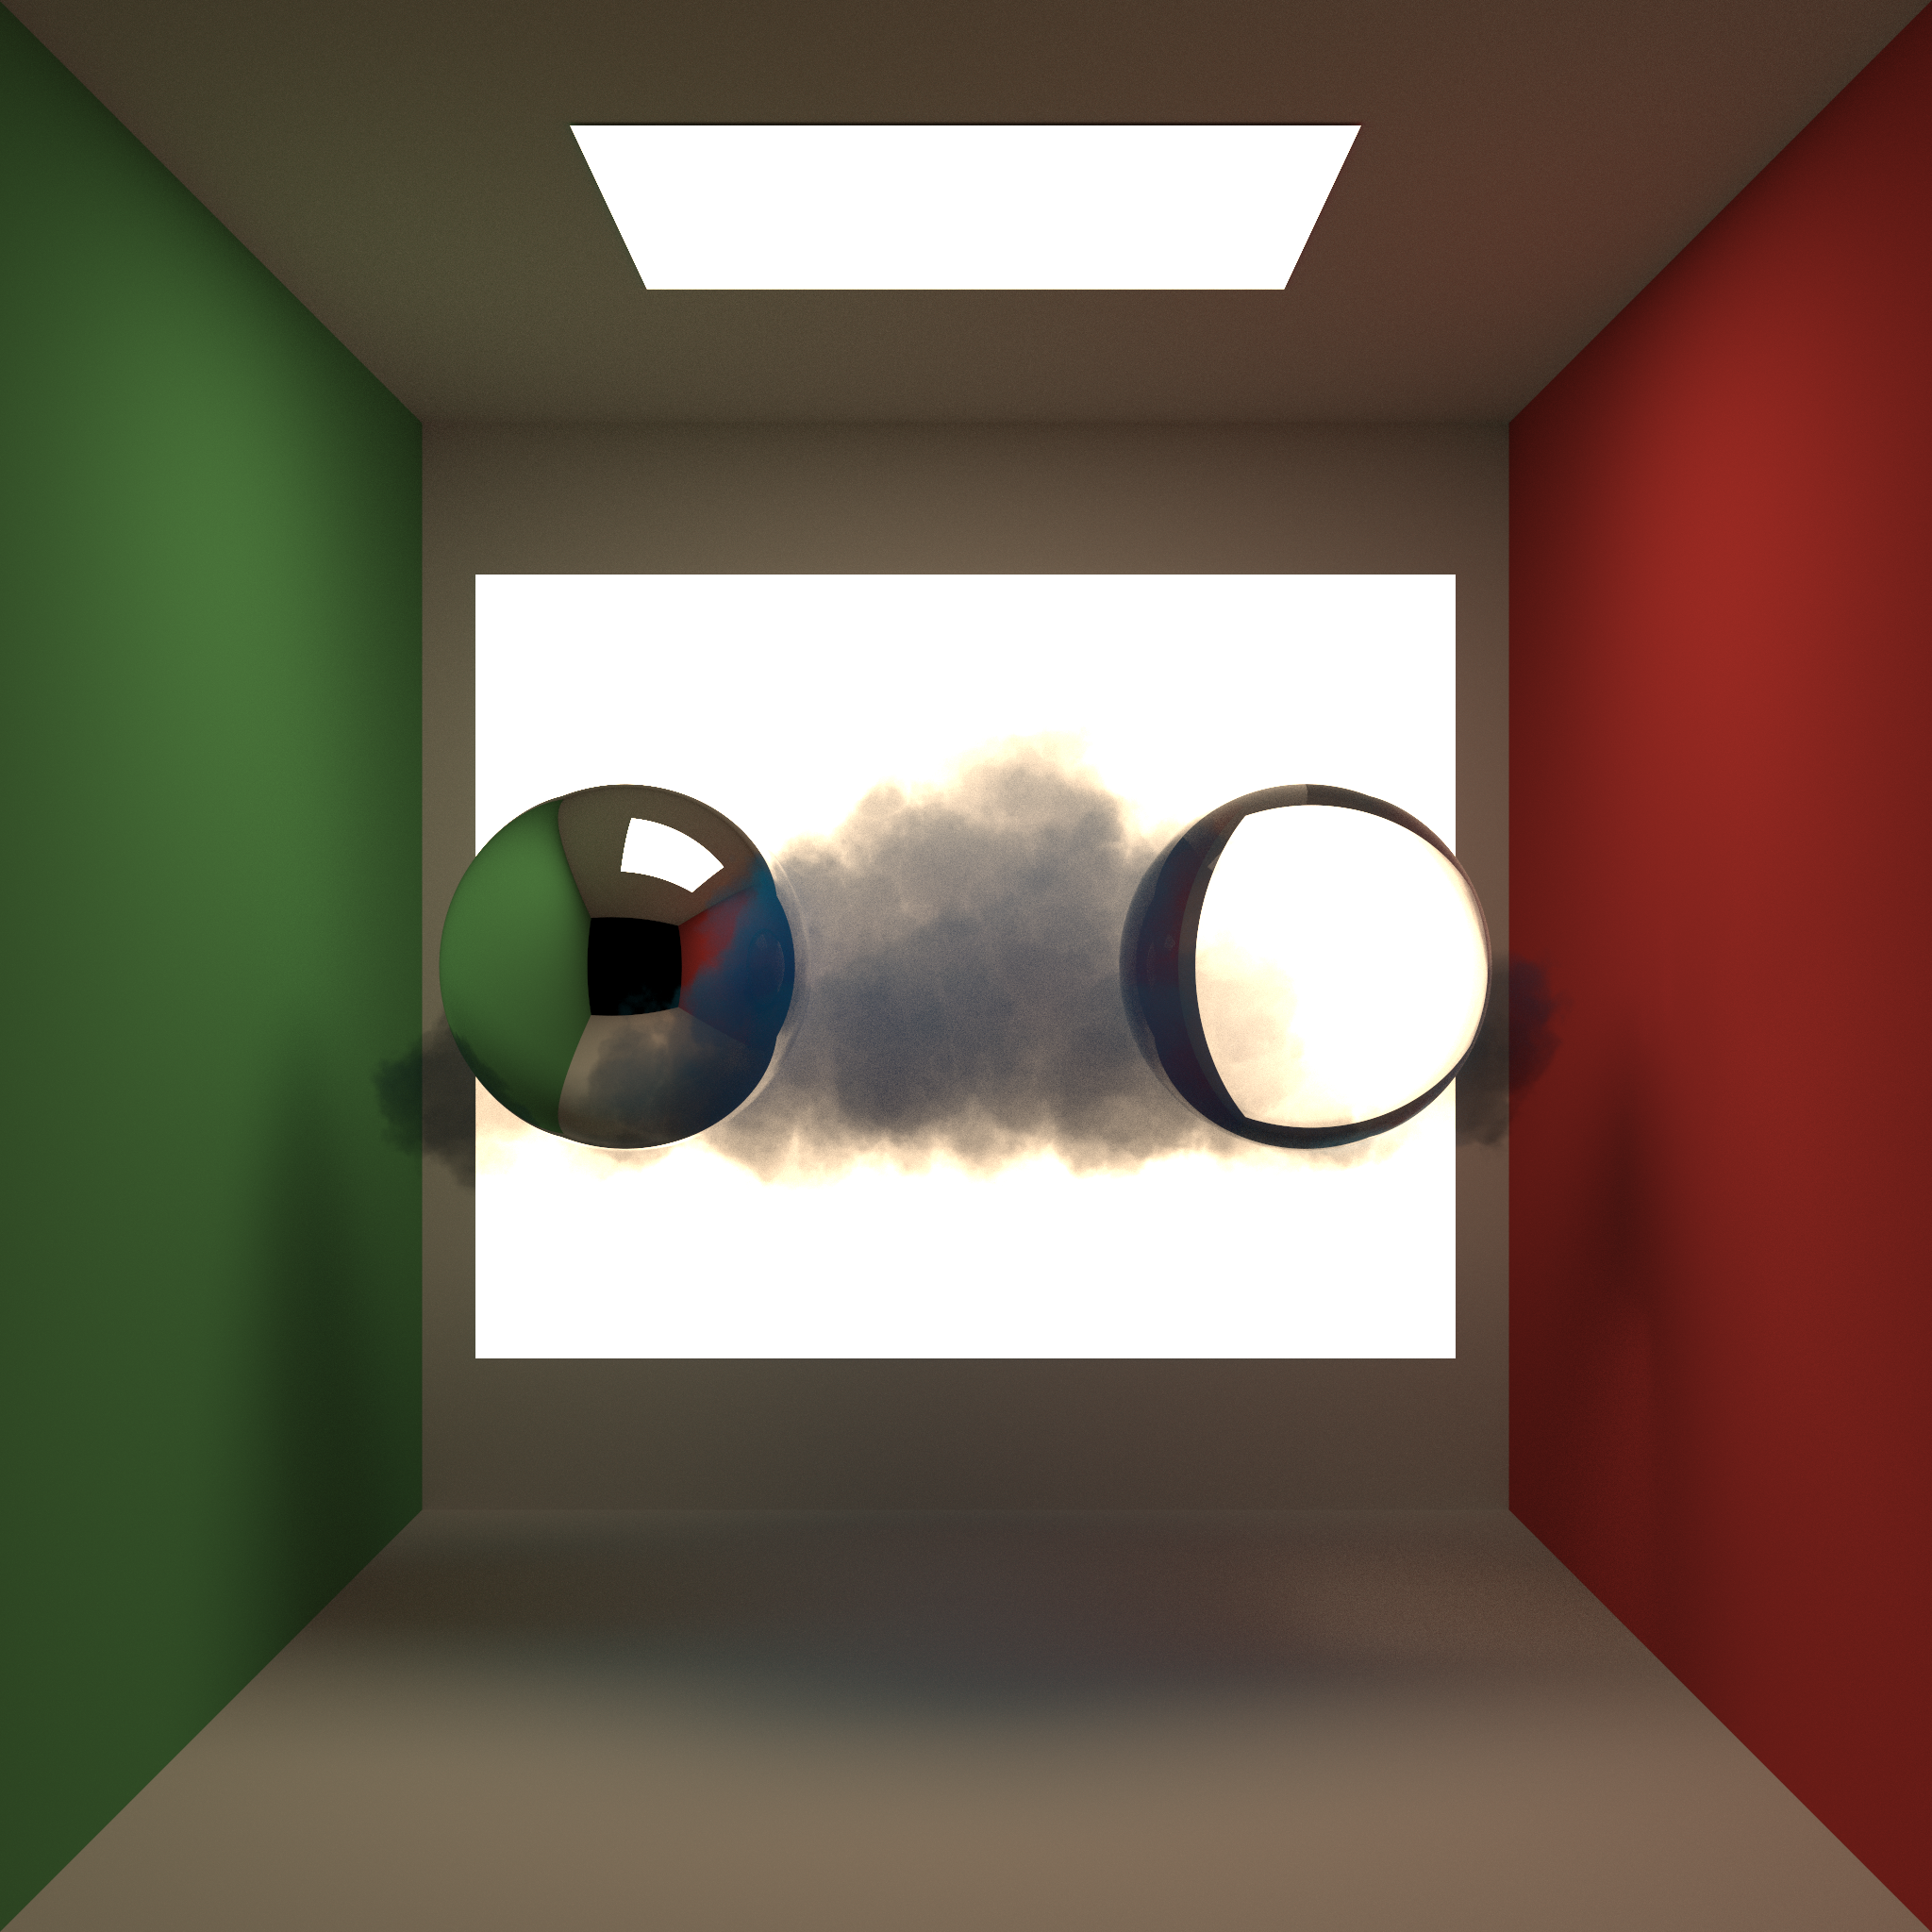
\includegraphics[width=\linewidth]{image2.png}
\end{figure}


\section{Contribution}
\paragraph{Yiheng Wu} The realization of the main part of the project:integrator,\\kdtree structure for volume, delta tracking and decomposition tracking. The implementation part of the report.
\paragraph{Haizhao Dai} Setting up many scenes for the project.Build up thread-safe random number generator. The learning and test experiment of Embree repo. The introduction part and first two sections of the theoretical part of the report.
\paragraph{Xiaohan Wu} Setting up many scenes for the project.The implementation of several API,including the loader of openvdb, surface-related interfaces. The arrangement of past and present codes(eg.light etc). The collection of openvdb assets.The last two sections of the theoretical part of the report.
\end{document} 
